\chapter{\label{cha:evaluation}Evaluation}
\section{Approach}
In this section, we run Cascaded 2-way Join, Multi-way Join, and modified Dan Suciu's Algorithm against 35 queries selected from Alibaba Benchmark and compare the performance. The RPQs are translated into DFA by library \cite{hackingoff} from HackingOff.com, which implements Thompson's construction algorithm \cite{Thompson:1968:PTR:363347.363387}. We eliminate the complex queries which take more than 1 hour sequentially. The queries selected can take 10 seconds at least, and in average 1 minute sequentially. The program is deployed to cluster with 2, 4, 8, 16, 32 and 64 executors on Surf Sara. Unfortunately, sometimes the tasks were too heavy for 2 or 4 machines, leading to a zookeeper timeout/crash, which returns no result. So those parts were ignored when gathering data.
\section{Metrics}
The experiment data is collected from the Spark UI and event logs, and the metrics we focus on are:
\begin{enumerate}
    \item Running time: The time spent on evaluating a single query, including both executor and driver sides while taking parallelism into account. At the same time, we count average duration, maximum duration and minimum duration spent on a single query.
    \item Time Stack: By analyzing the event log of spark applications, the application runtime can be split into several parts:
        \begin{enumerate}
        \item Executor Computing Time: The average time each executor spends on the computation of action or transform steps.
        \item Shuffle Read/Write Time: The average time each executor spends on writing or reading shuffled data.
        \item Transforming Time: The average time each executor spends on de-serializing the tasks and serializing result.
        \item Scheduler Delay Time: The average time it takes to send task from scheduler to executor.
        \item JVM GC Time: The time spent on garbage collection.
        \end{enumerate}
    \item Shuffled data size: Most disk I/O and network communications happen during data shuffling. During shuffling data, Spark executors will write data to the local buffer in shuffle write phase, and based on the key of requested data, each executor reads data from the local buffer or remote buffer of other executors. 
    % \item Memory usage: We measure the peak memory usage of all executors. As Spark is a memory-based computing framework, it's crucial to monitor memory usage and avoid spilling data to disk, which would impact the performance.
\end{enumerate}
\section{Running Time}
Figure \ref{fig:Average-RunTime-for-Each-Alibaba-Query} depicts running time stats for those queries:
\begin{figure}[h!]
  \caption{Average Running Time Comparison}
  \label{fig:Average-RunTime-for-Each-Alibaba-Query}
  \centering
    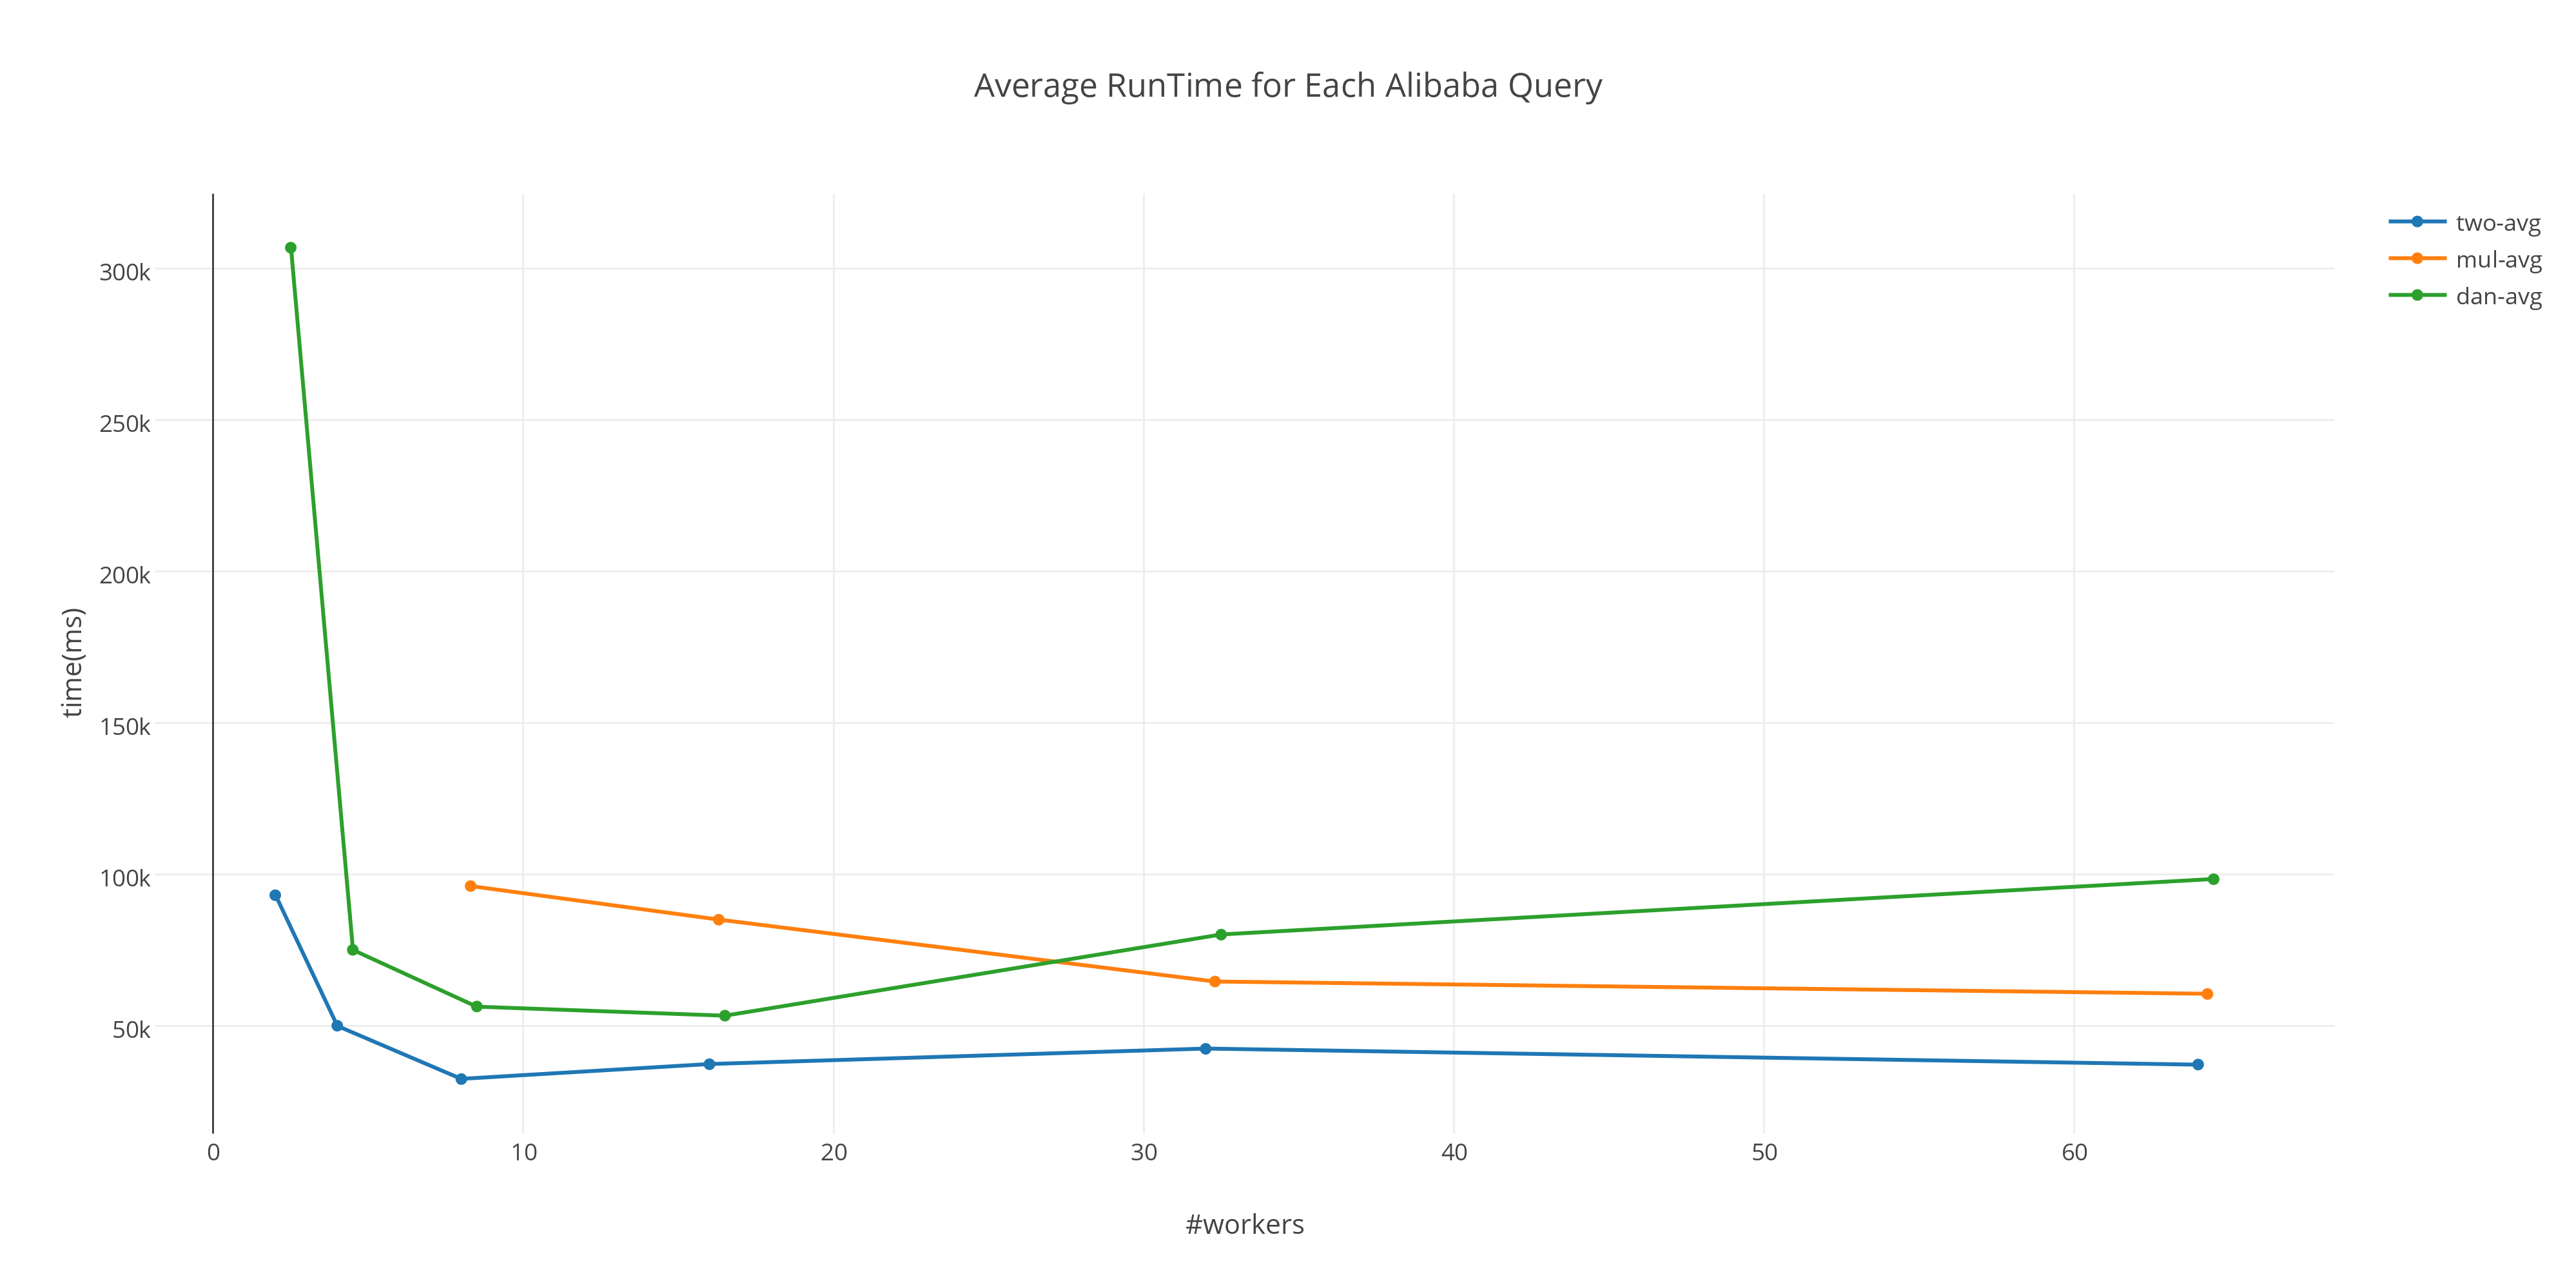
\includegraphics[width=1.0\textwidth]{img/Average-RunTime-for-Each-Alibaba-Query}
\end{figure}
\\The figure suggests cascaded two-way join is the most scalable and fastest solution for this benchmark. Dan Suciu's algorithm also has good speed up when the number of executors is less than 10. When the executor number is larger, the overhead introduced cannot be made up by speed-up already.
\begin{figure}[h!]
  \caption{Average Running Time of Two-Way Join}
  \label{fig:two-way-join-general}
  \centering
    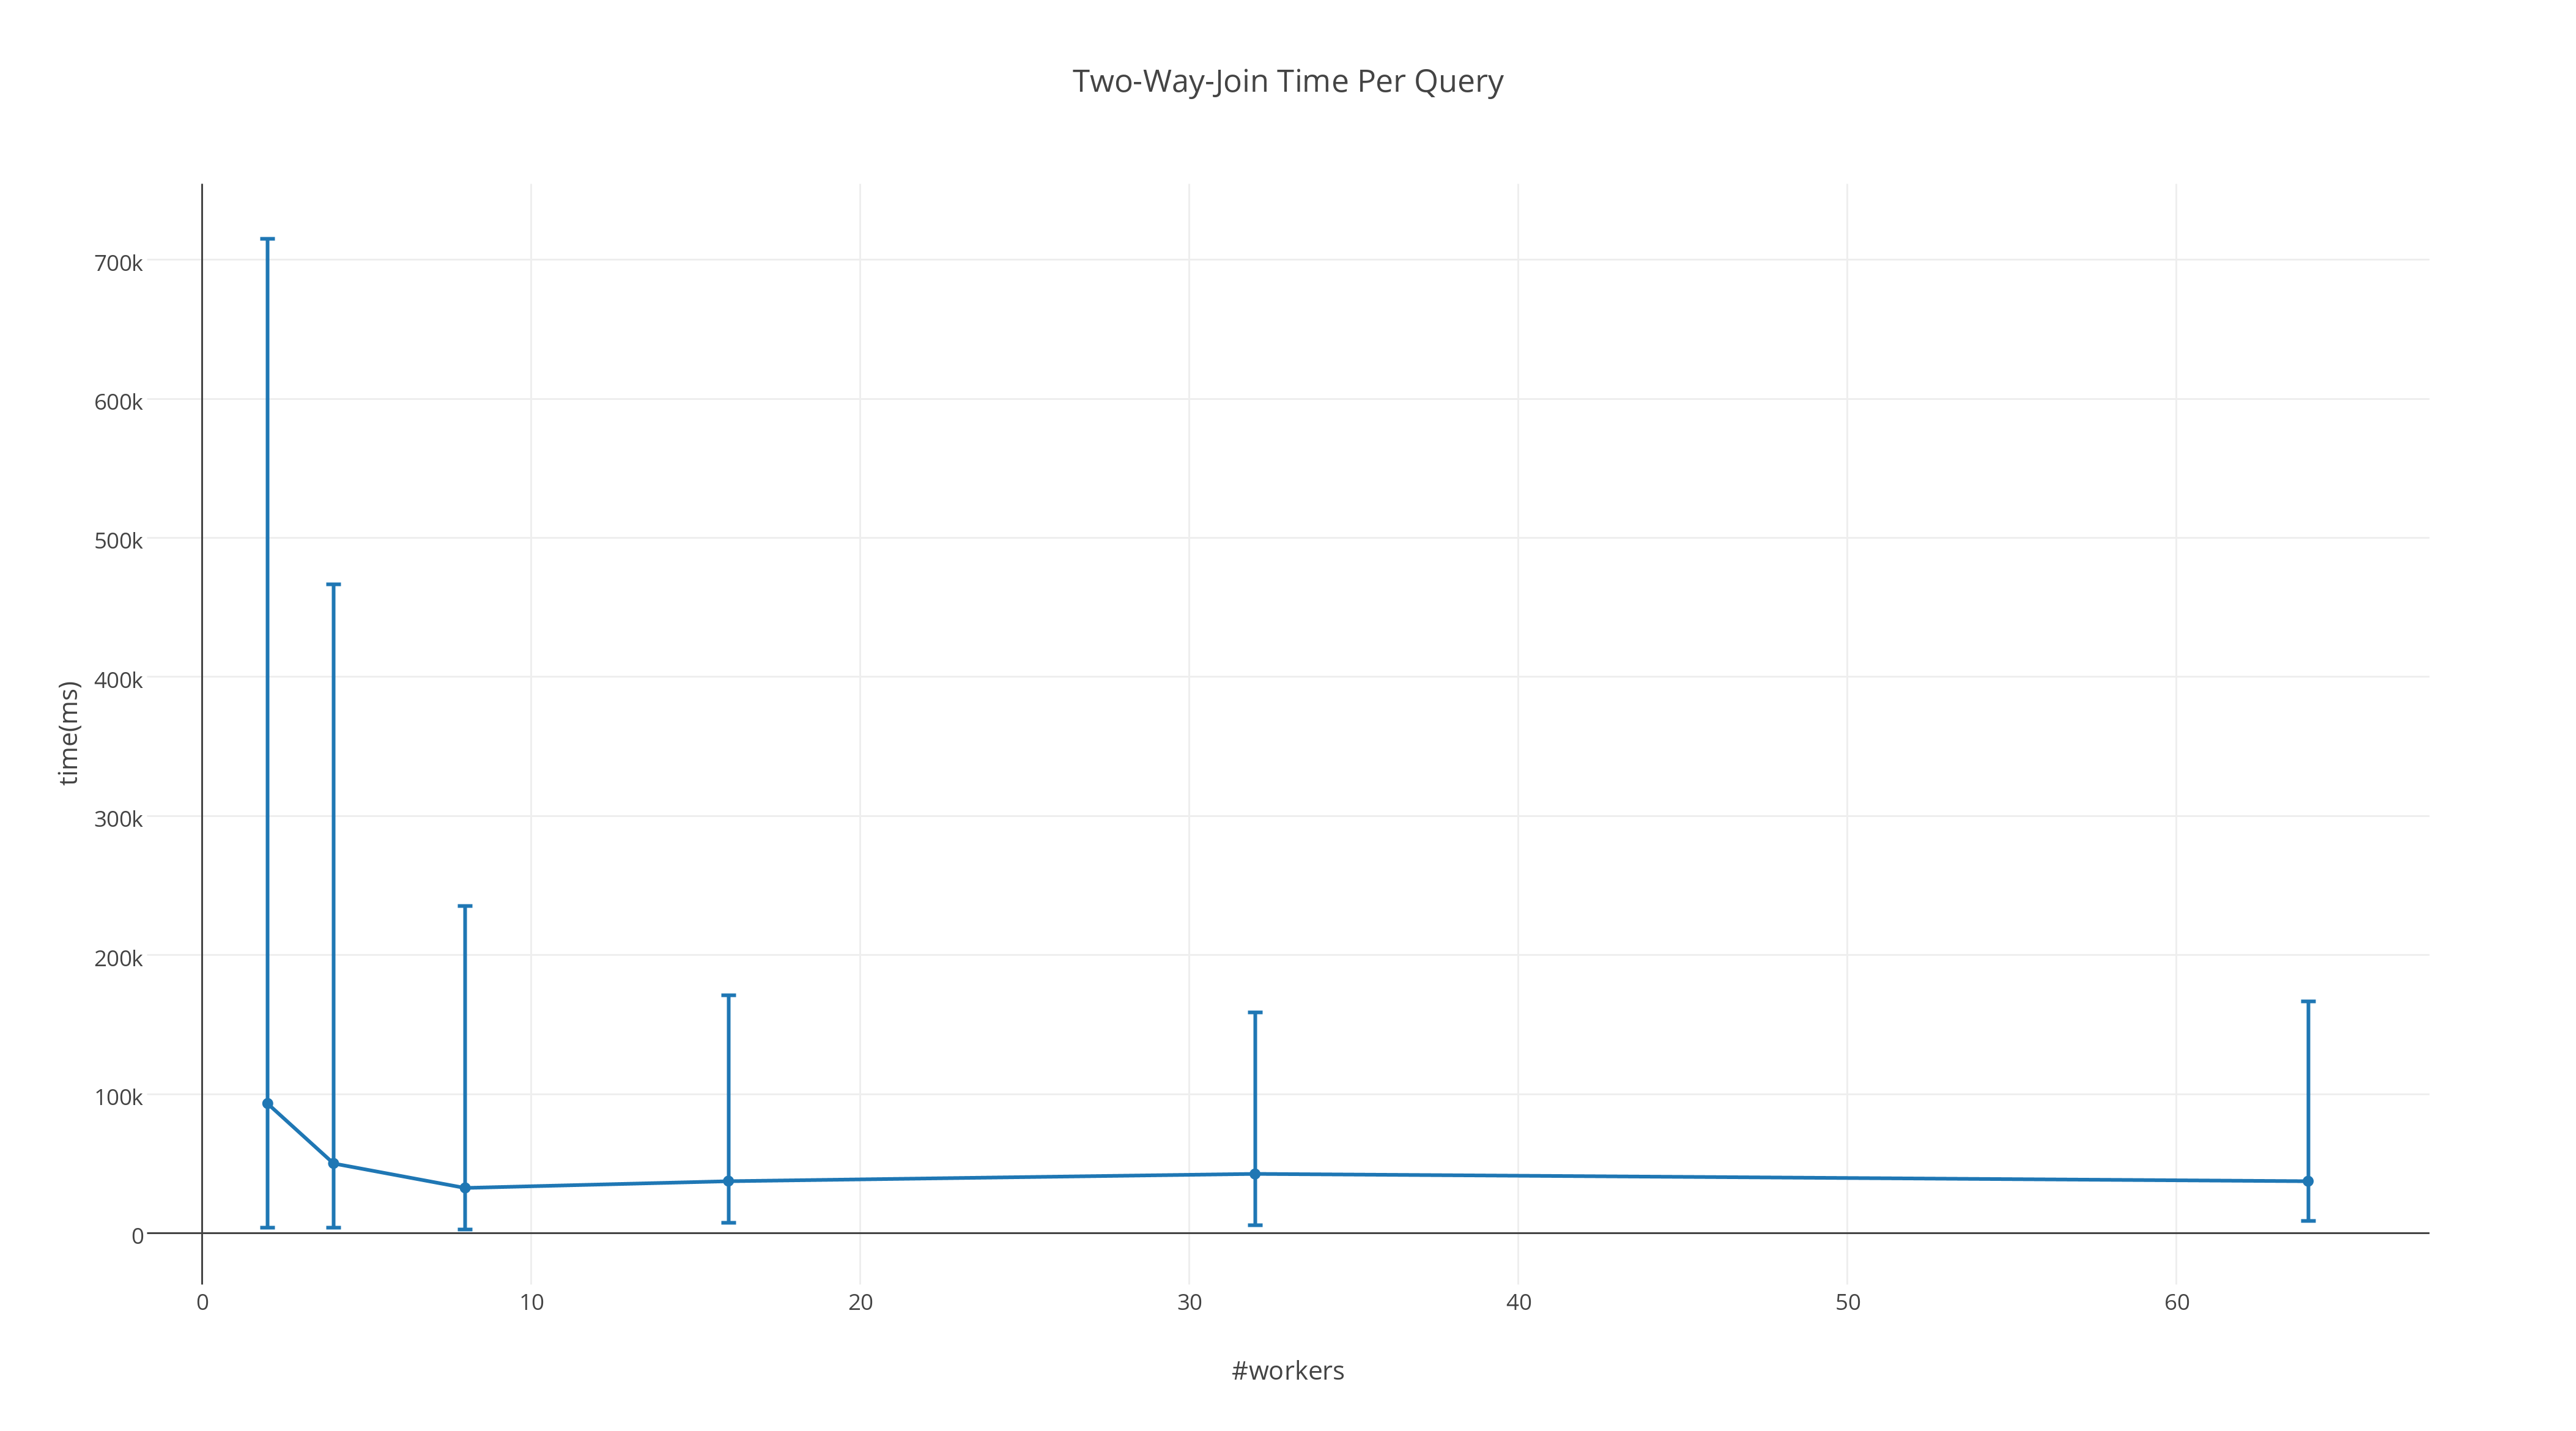
\includegraphics[width=1.0\textwidth]{img/Two-Way-Join-General}
\end{figure}
\begin{figure}[h!]
  \caption{Average Running Time of Multi-Way Join}
  \label{fig:multi-way-general}
  \centering
    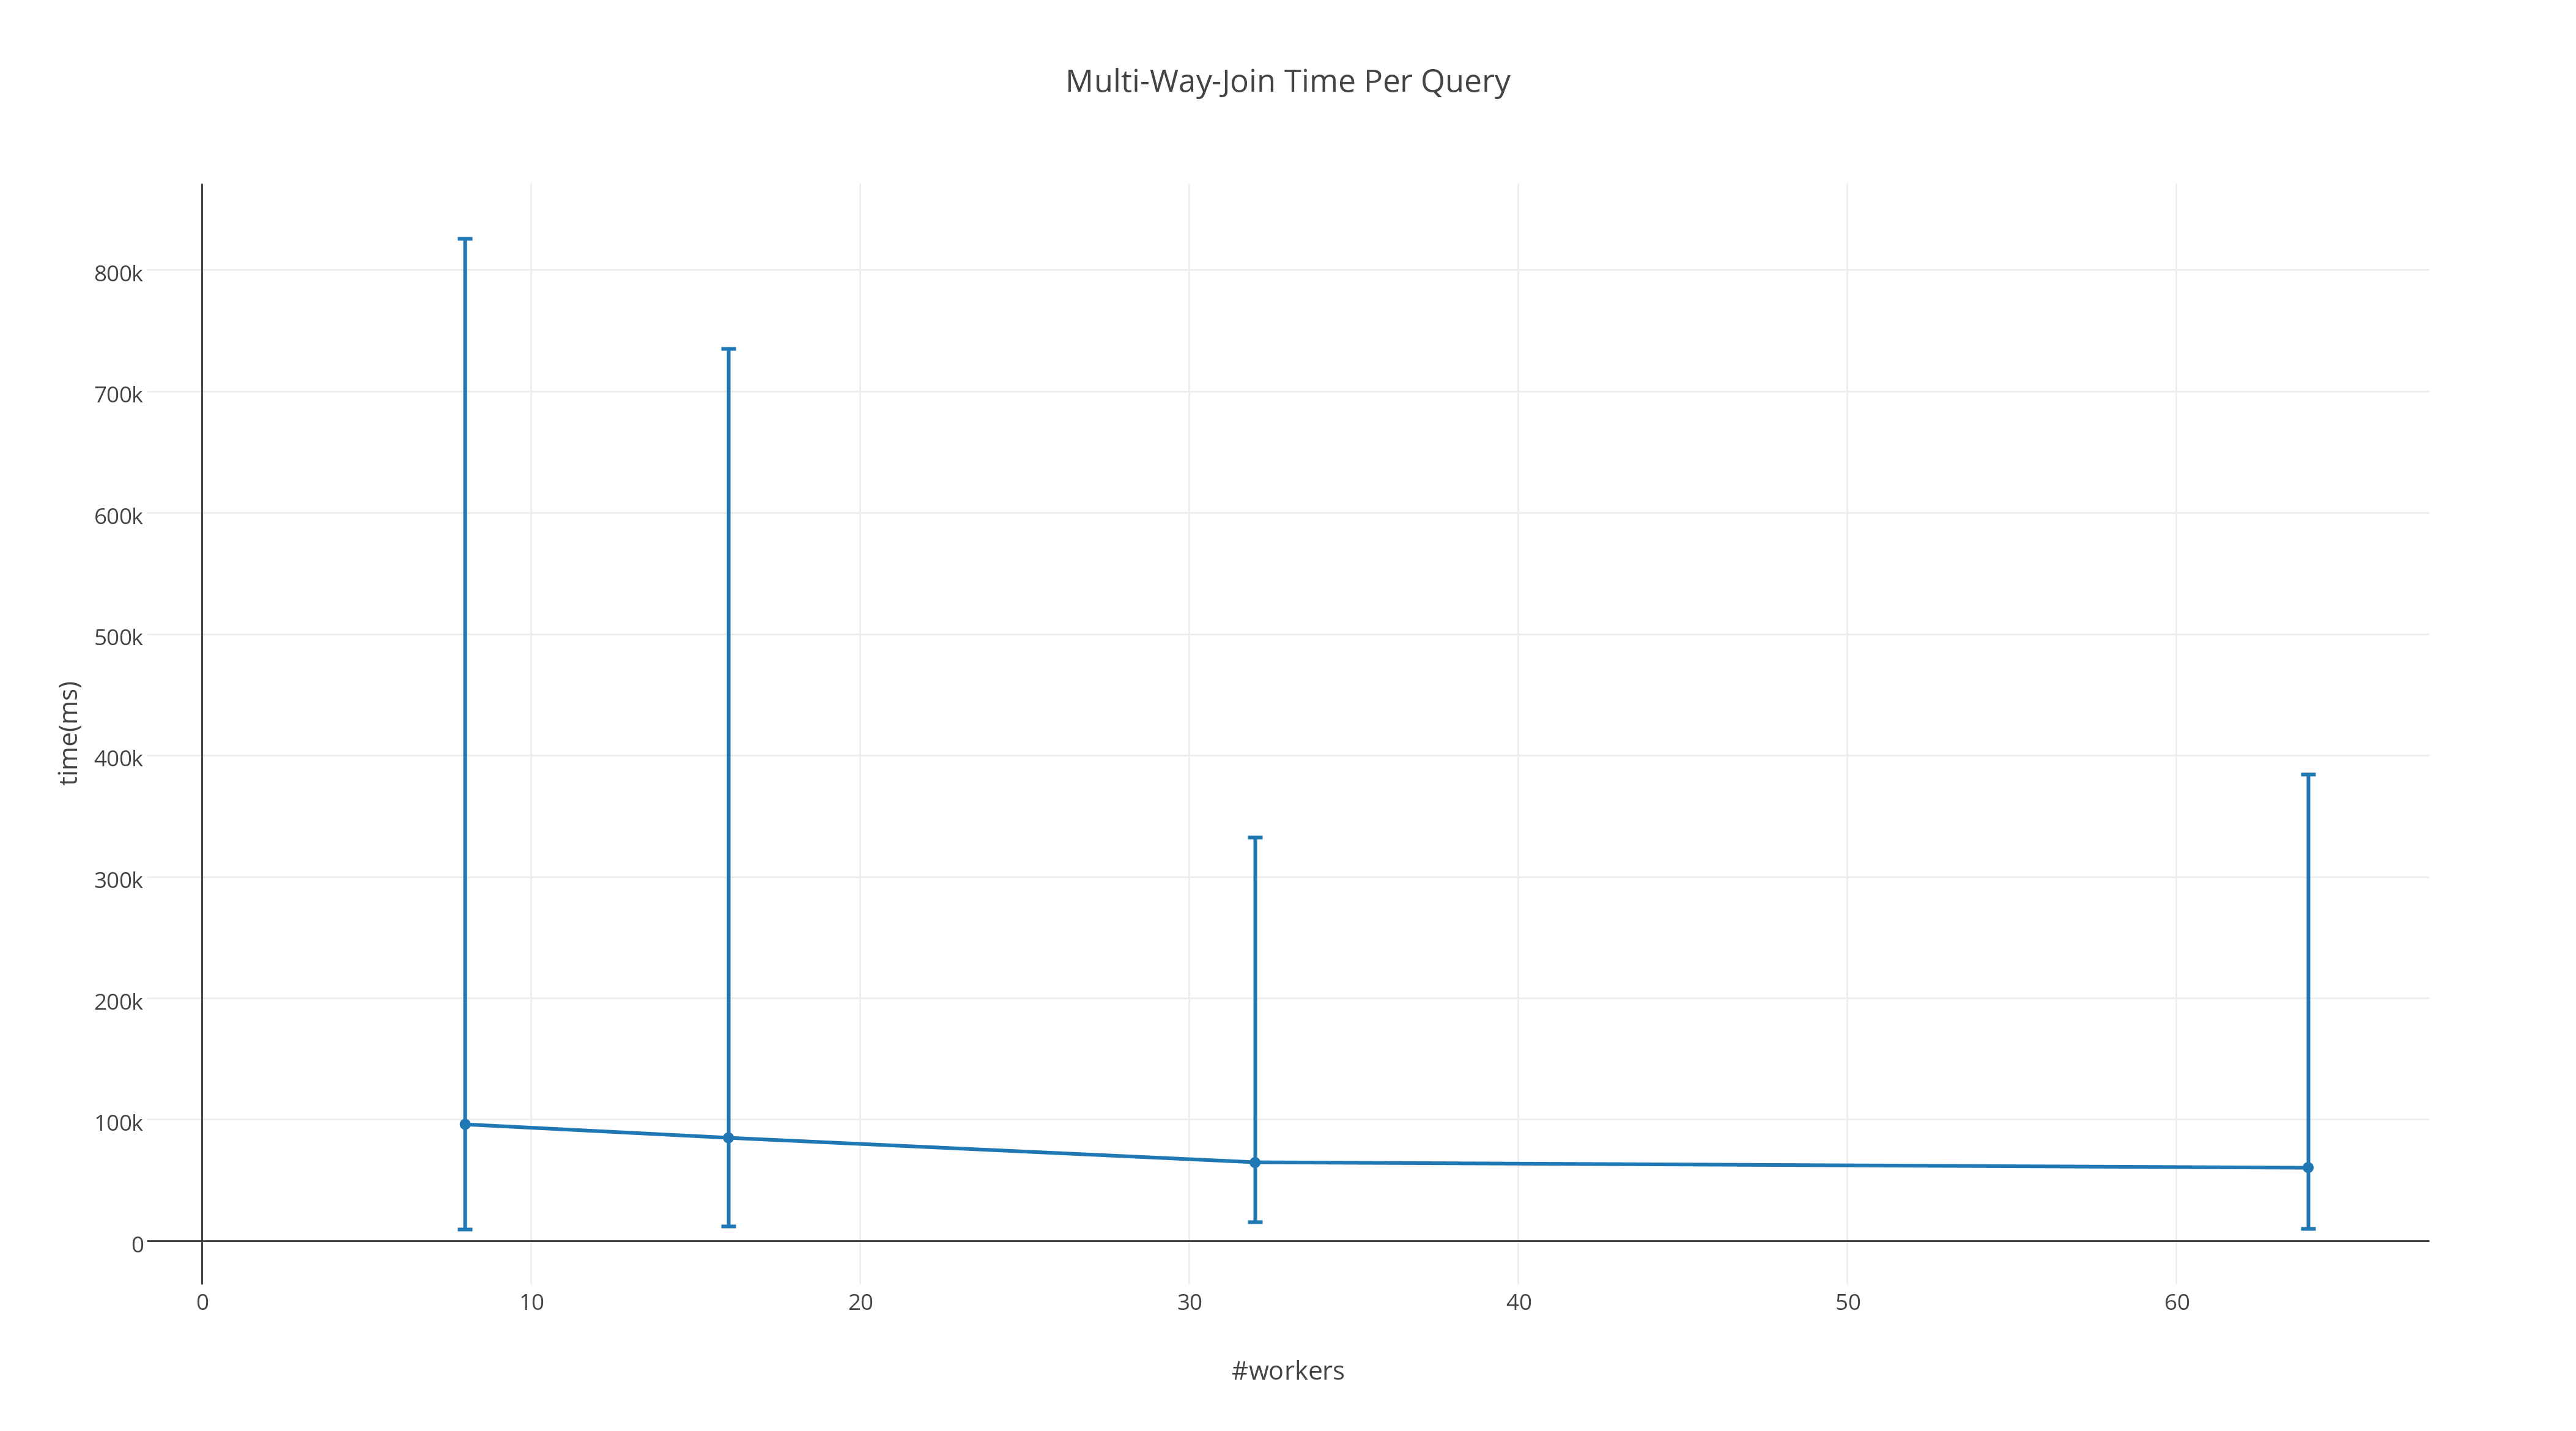
\includegraphics[width=0.8\textwidth]{img/Multi-Way-Join-General}
\end{figure}
\begin{figure}[h!]
  \caption{Average Running Time of Modified Dan Suciu's Algorithm}
  \label{fig:Dan-Algorithm-General}
  \centering
    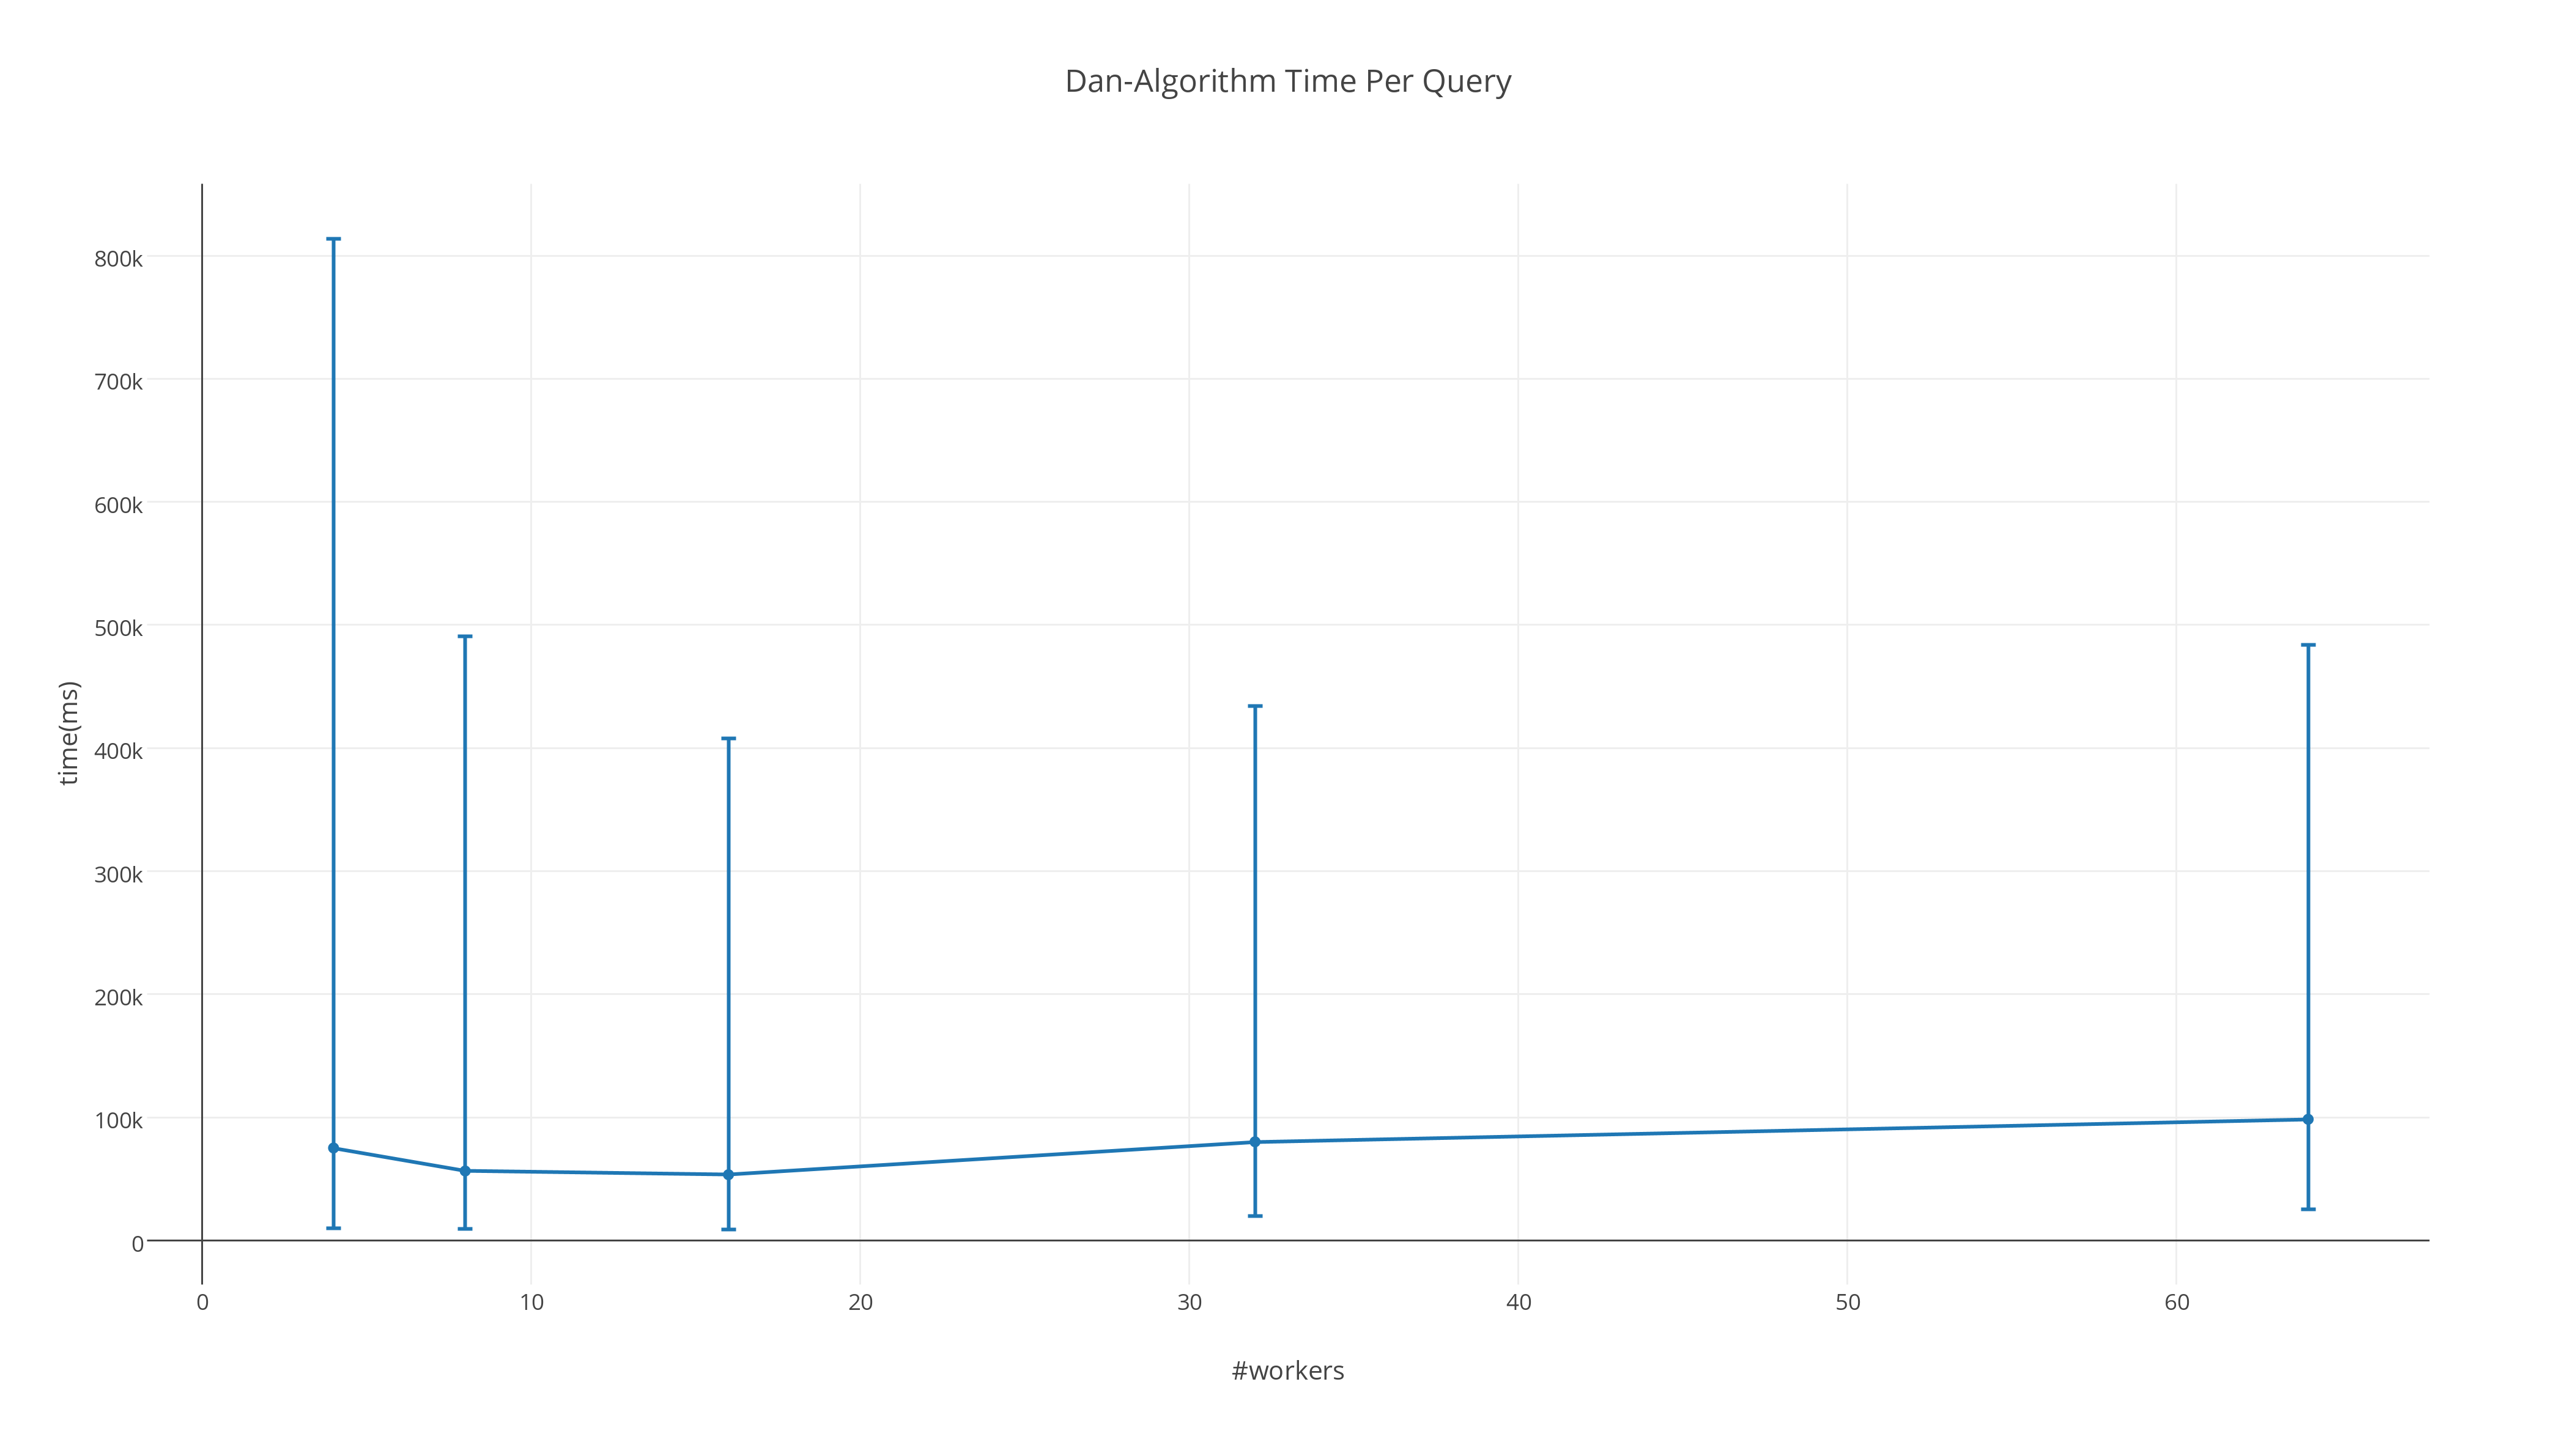
\includegraphics[width=0.8\textwidth]{img/Dan-Algorithm-General}
\end{figure}
\\From the Figure \ref{fig:two-way-join-general} and Figure \ref{fig:multi-way-general} we can see that each query takes around one minute in average. The difference between maximum values of different number of processors indicates that there is a small part of queries which take much longer time. This can be improved significantly by adding more workers. The time spent on a long query is still decreasing with 16 workers while minimum time increases, which in total makes average time higher as there are more simple queries. 
\\Average Running Time for Dan Suciu's algorithm goes up after 16 workers since the graph is split into slight pieces, and there is less chance to do the local search on each partition. In this case, more computation happens on the driver side with more small fragments, which increases the running time. This phenomenon will be discussed further in next chapter.
\\In general, for this data and query size, the running time is already very short, so that introducing more computation power cannot make up with the overhead brought by it. The evidence for this can be found in the next section.
\section{Time Stack}
\begin{figure}[h!]
  \caption{Time Stack of Two-Way Join}
  \label{fig:two-way-join-stack}
  \centering
    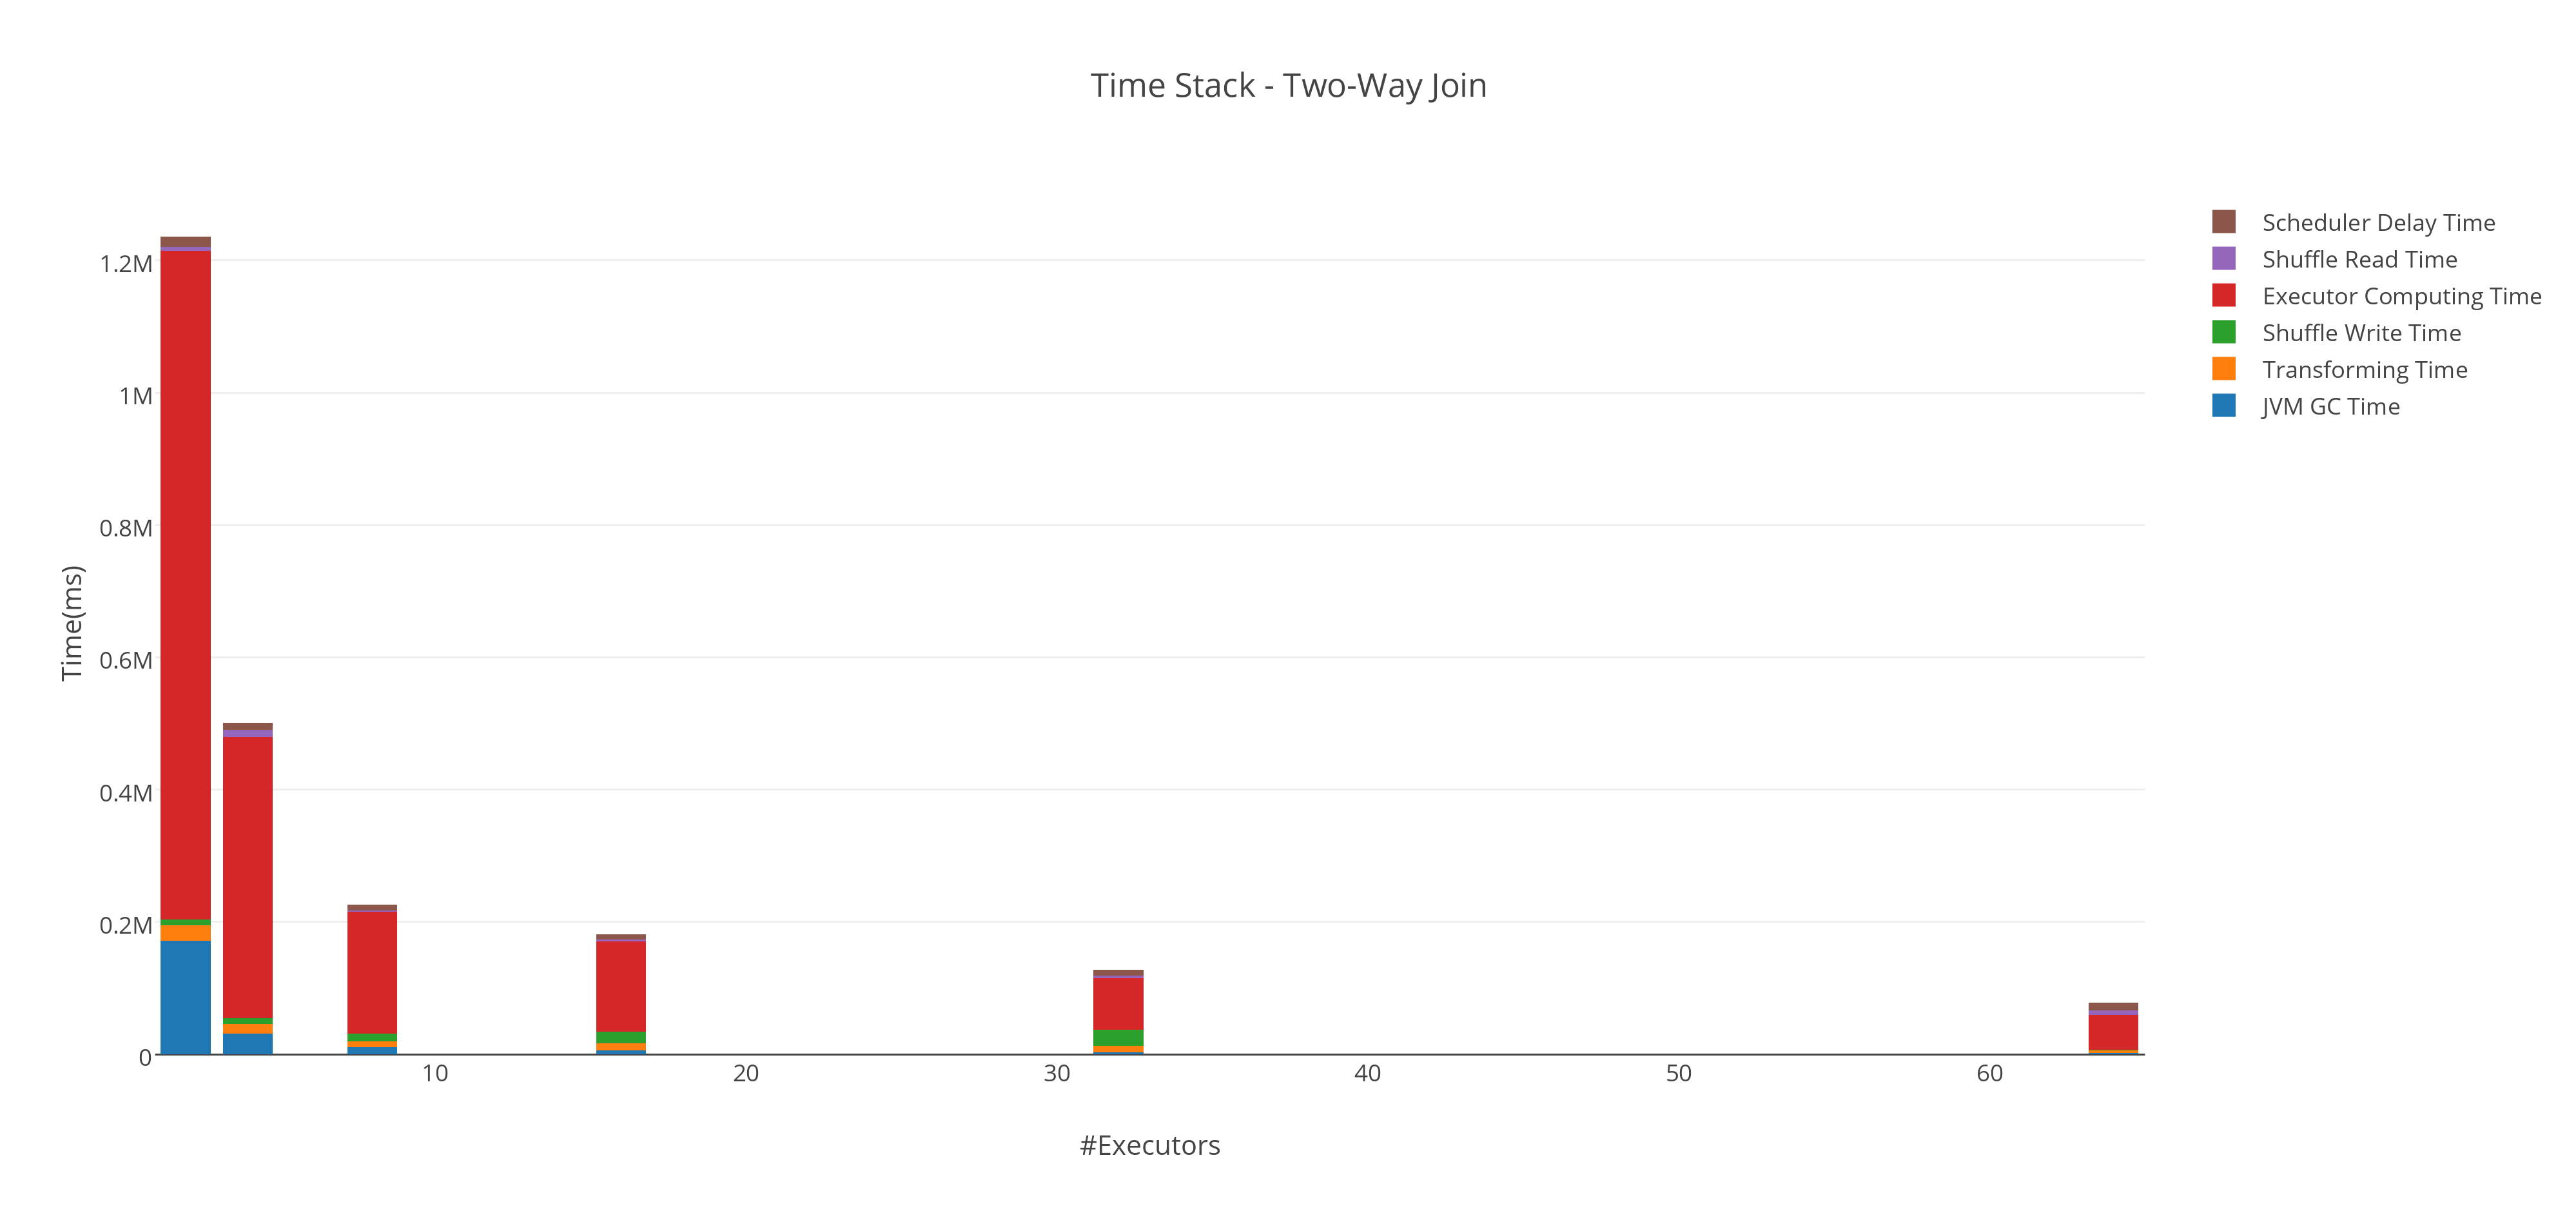
\includegraphics[width=1.0\textwidth]{img/Timestack-twoway}
\end{figure}
\begin{figure}[h!]
  \caption{Time Stack of Multi-Way Join}
  \label{fig:timestack-multiway}
  \centering
    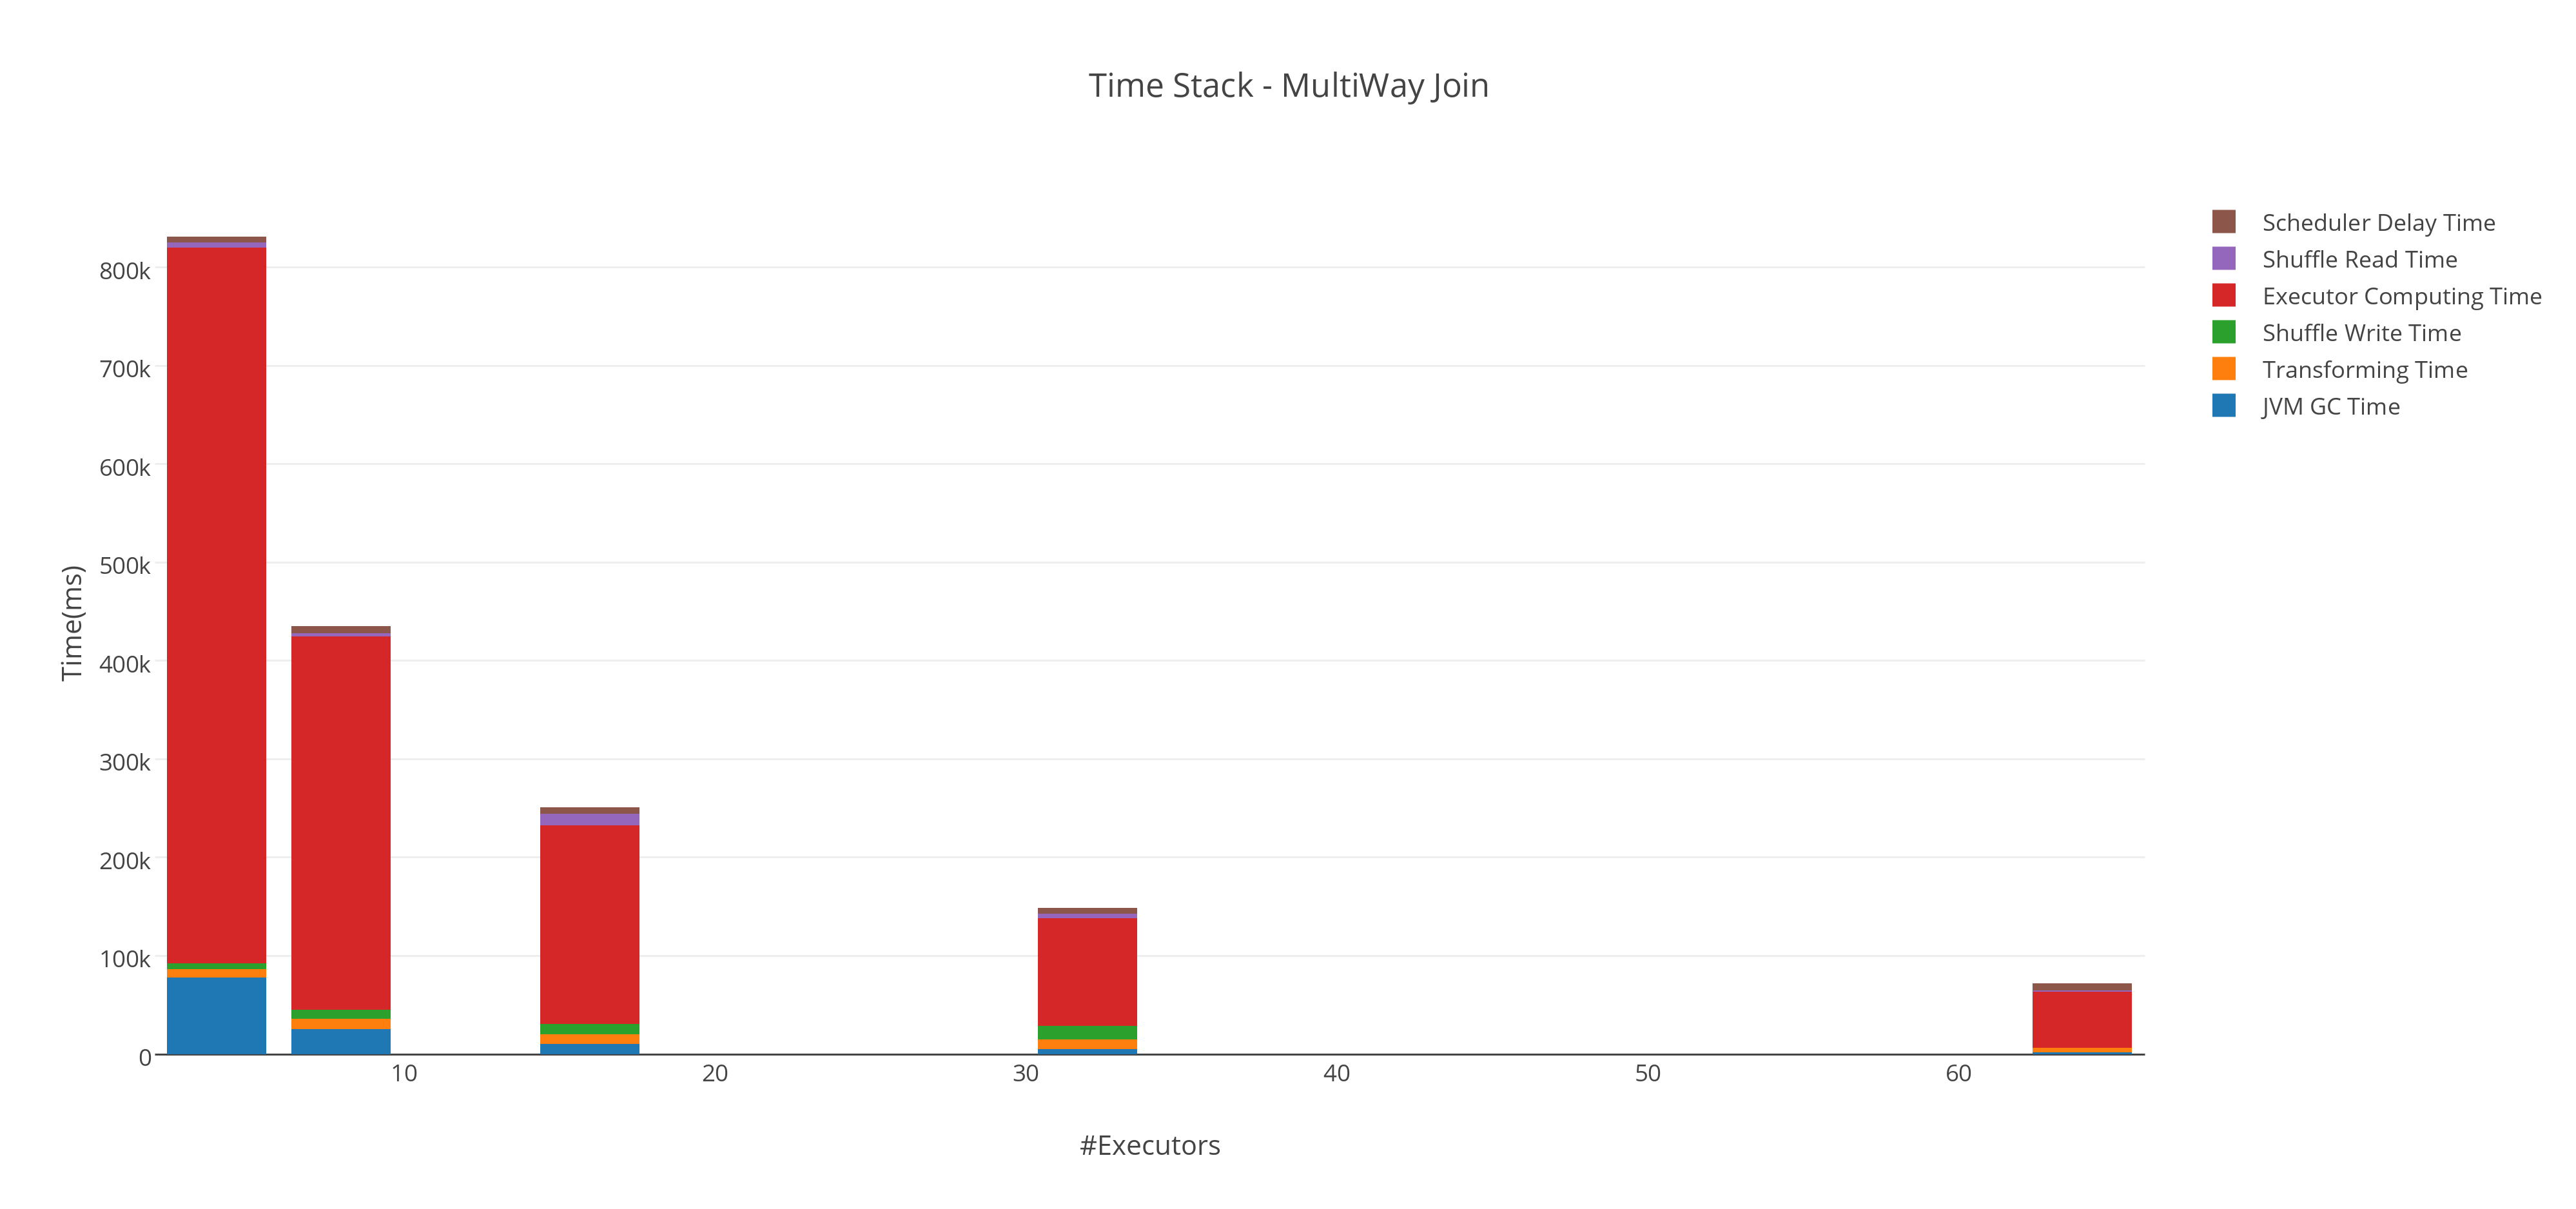
\includegraphics[width=0.8\textwidth]{img/Timestack-multiway}
\end{figure}
According to the diagrams \ref{fig:two-way-join-stack} and \ref{fig:timestack-multiway}, the average executor computing time is always decreasing after adding more workers. Specifically, the time spent on computing is quite small when the number of workers is 64. The reason behind those trends being different from the ones in figure  \ref{fig:two-way-join-general} and figure \ref{fig:multi-way-general} is that tasks are not evenly distributed on different executors, and the blocking time can not be revealed by the average time we measured here. The GC Time is also decreasing dramatically as with more workers as each executor would use less memory. Comparing to the blocking time, the time spent on writing and reading the shuffled data is relatively ignorable, although they are also increasingly slow. The time stack for Dan Scuciu's algorithm is not shown here as the actual running time for each executor is less than $1/10$ of the total time, which will be discussed in bottleneck part.\\
One reason the Multi-way Join is being slower than cascaded two-way join is that the time difference between the busiest executor and idlest one is larger, which is revealed in diagram  \ref{fig:Time-Range-Difference-For-All-Executors.png}. The shuffle phases in the cascaded two-way join are scheduled by native spark function, which can dispatch tasks to processors evenly. However, because of the nature of the Multi-way Join, the size of different reducing tasks in the Multi-way Join can be very different, which explains the phenomenon that some executors are busy while others are just blocked and waiting for them.
\begin{figure}[h!]
  \caption{Maximum Blocking Time for Executors}
  \label{fig:Time-Range-Difference-For-All-Executors.png}
  \centering
    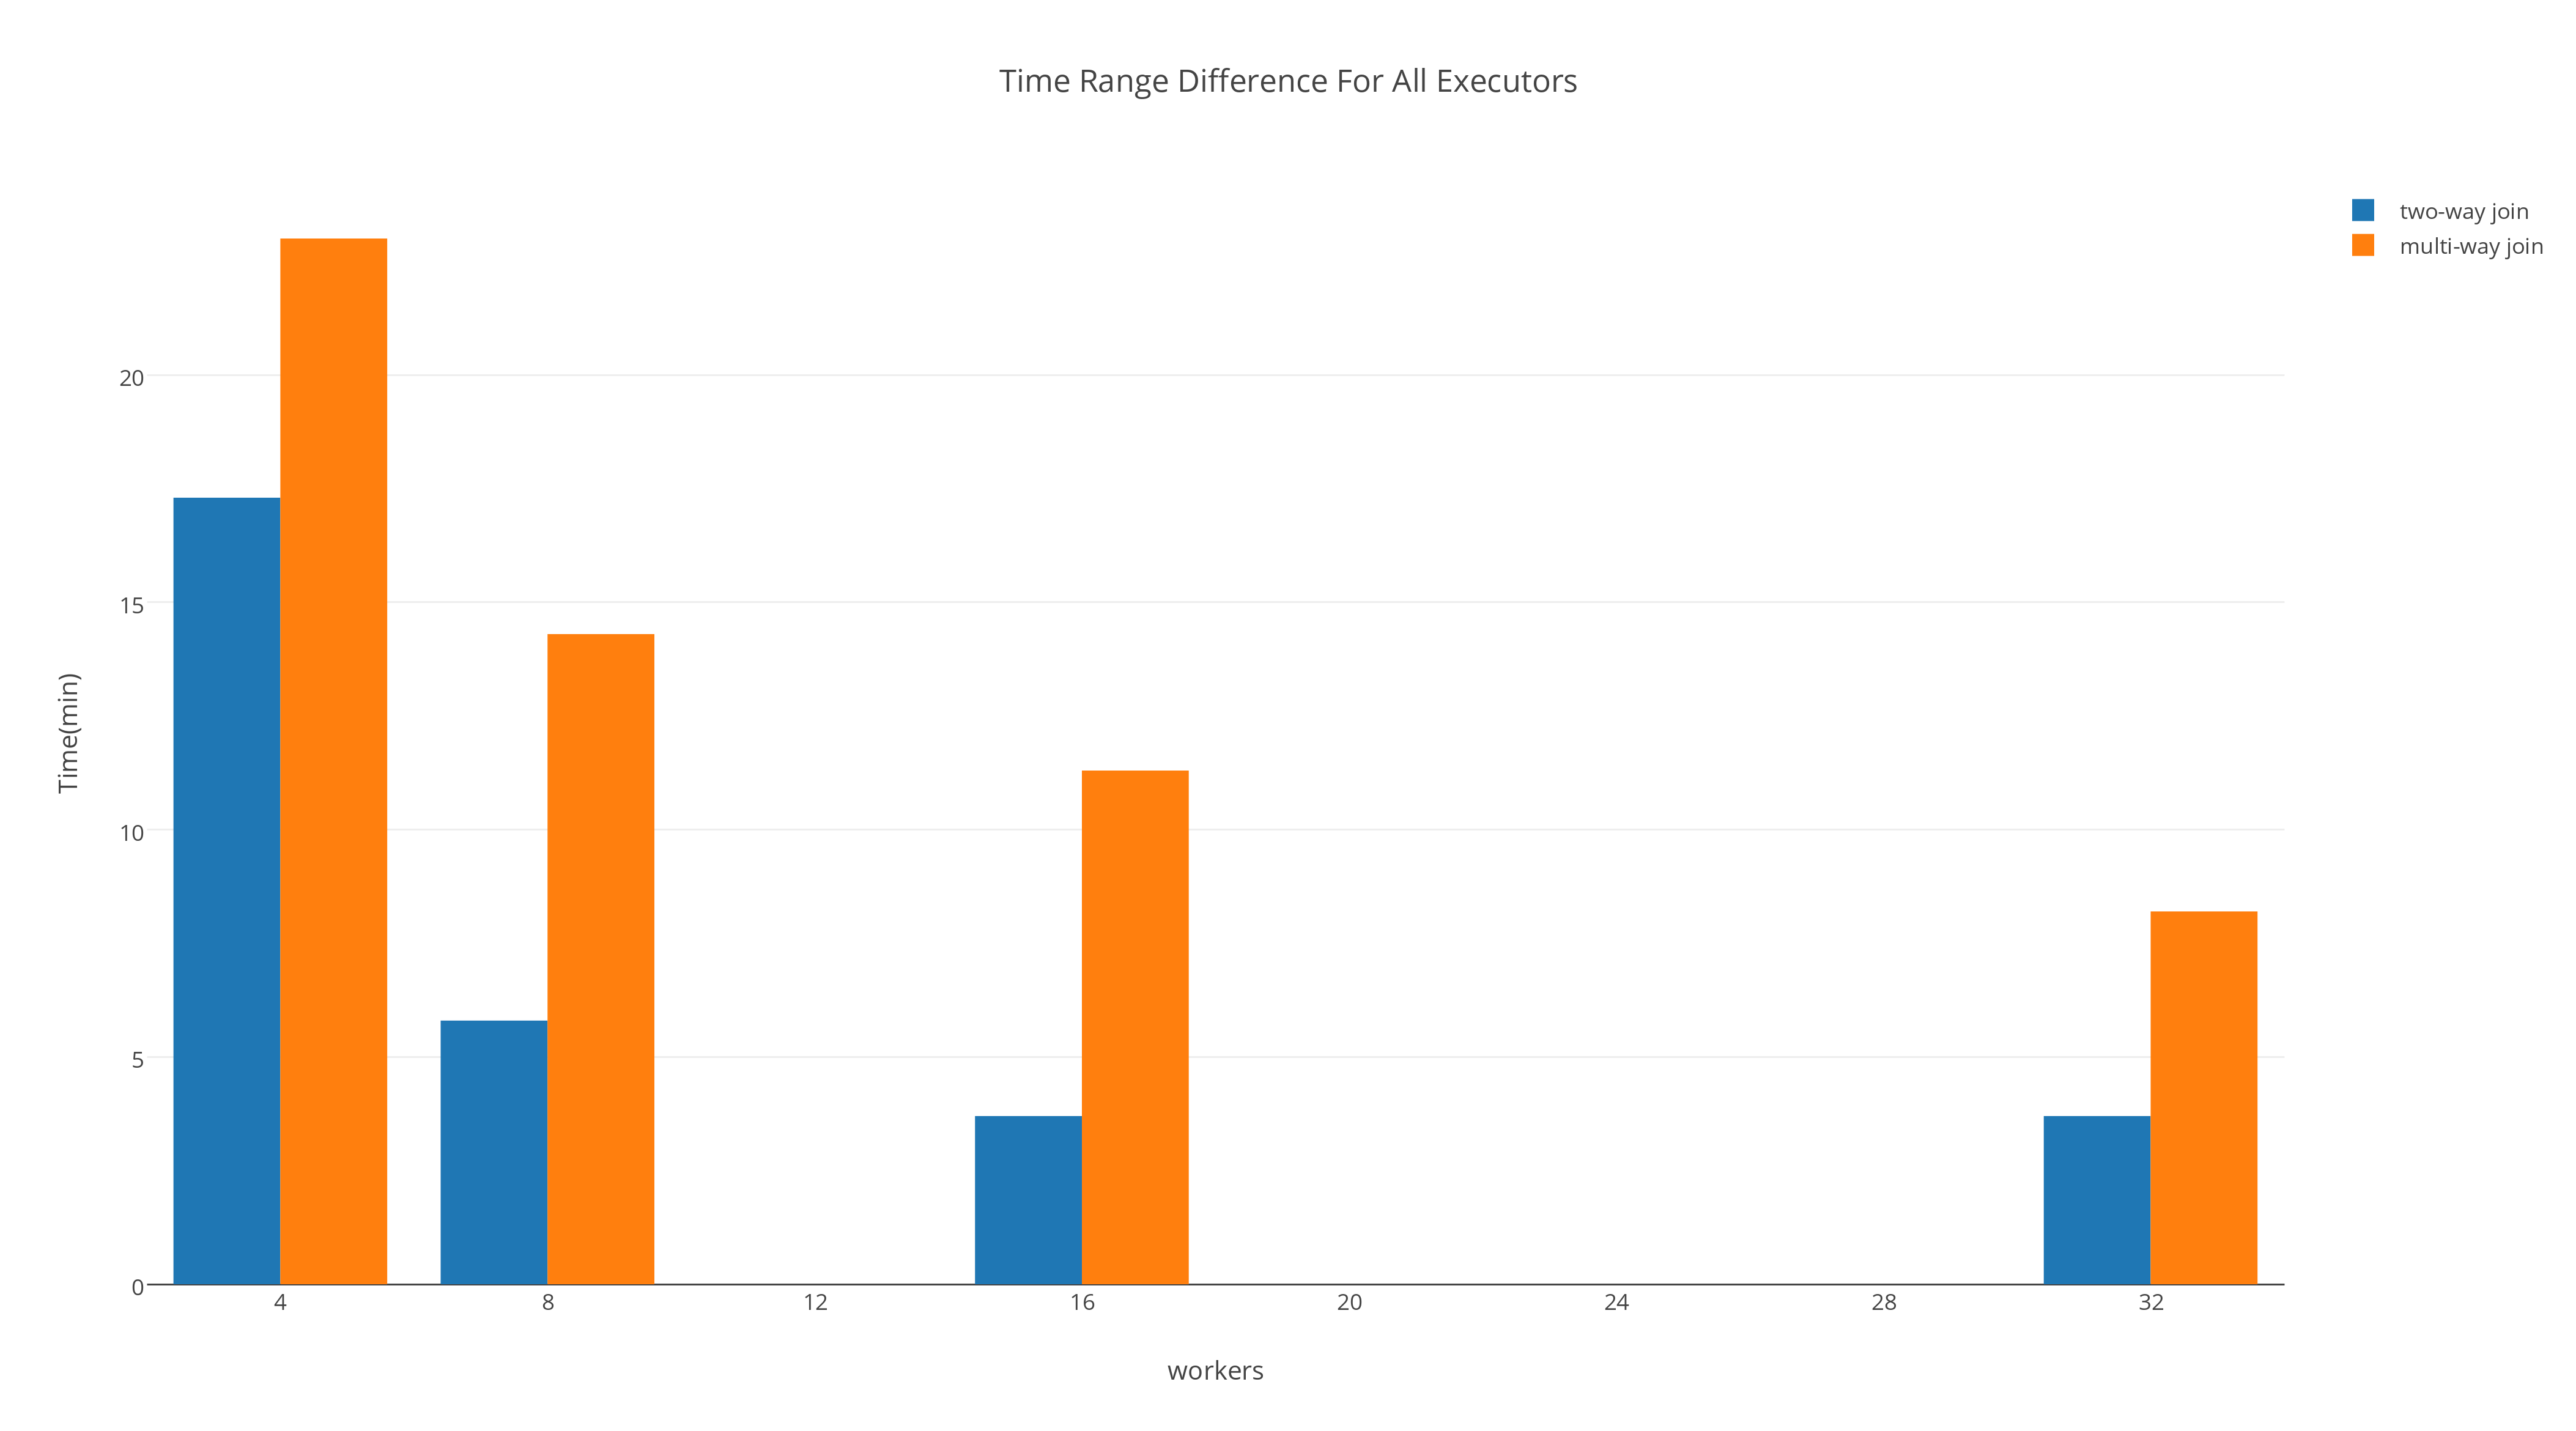
\includegraphics[width=0.8\textwidth]{img/Time-Range-Difference-For-All-Executors}
\end{figure}

\section{Bottleneck}
Furthermore, more insights are revealed by the job flow-chart in Spark Web-UI. The charts  \ref{fig:alibaba-two-jobs}, \ref{fig:alibaba-multi-jobs} and \ref{fig:alibaba-dan-jobs} present the status of different spark jobs along the time-line.
\begin{figure}[h!]
  \caption{Job Flow of Cascaded Two-Way Join}
  \label{fig:alibaba-two-jobs}
  \centering
    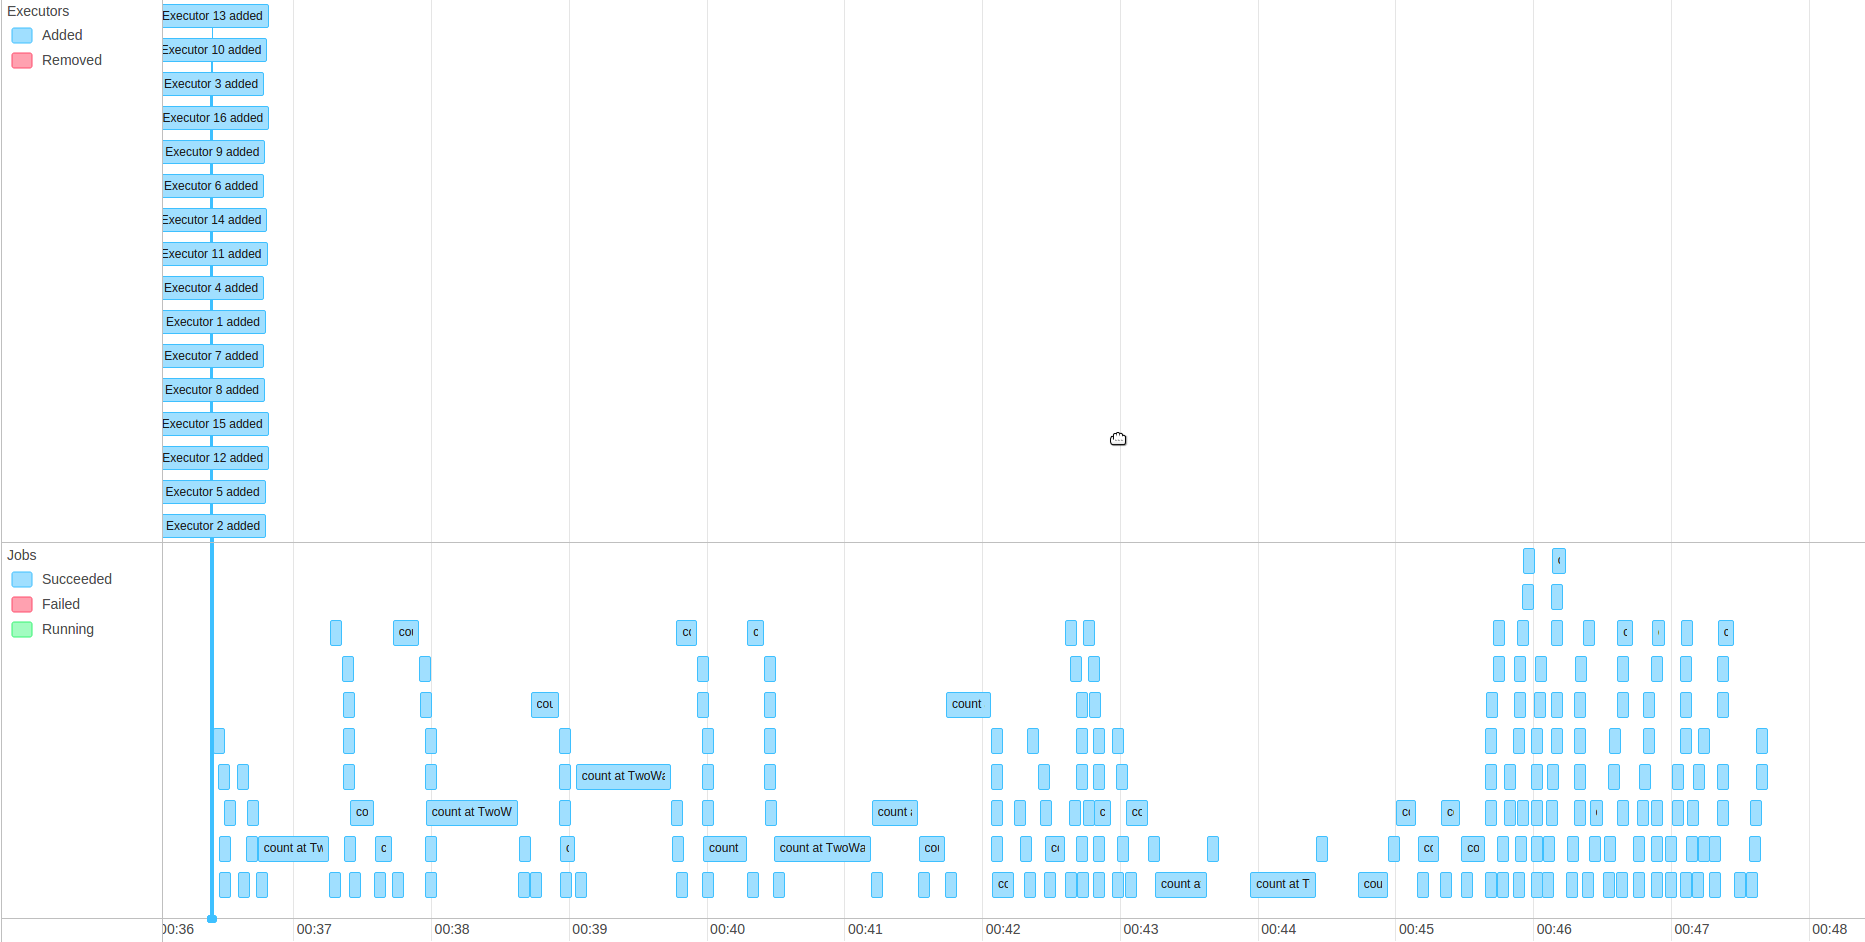
\includegraphics[width=1.0\textwidth]{img/alibaba-two-jobs}
\end{figure}
\begin{figure}[h!]
  \caption{Job Flow of Multi-Way Join}
  \label{fig:alibaba-multi-jobs}
  \centering
    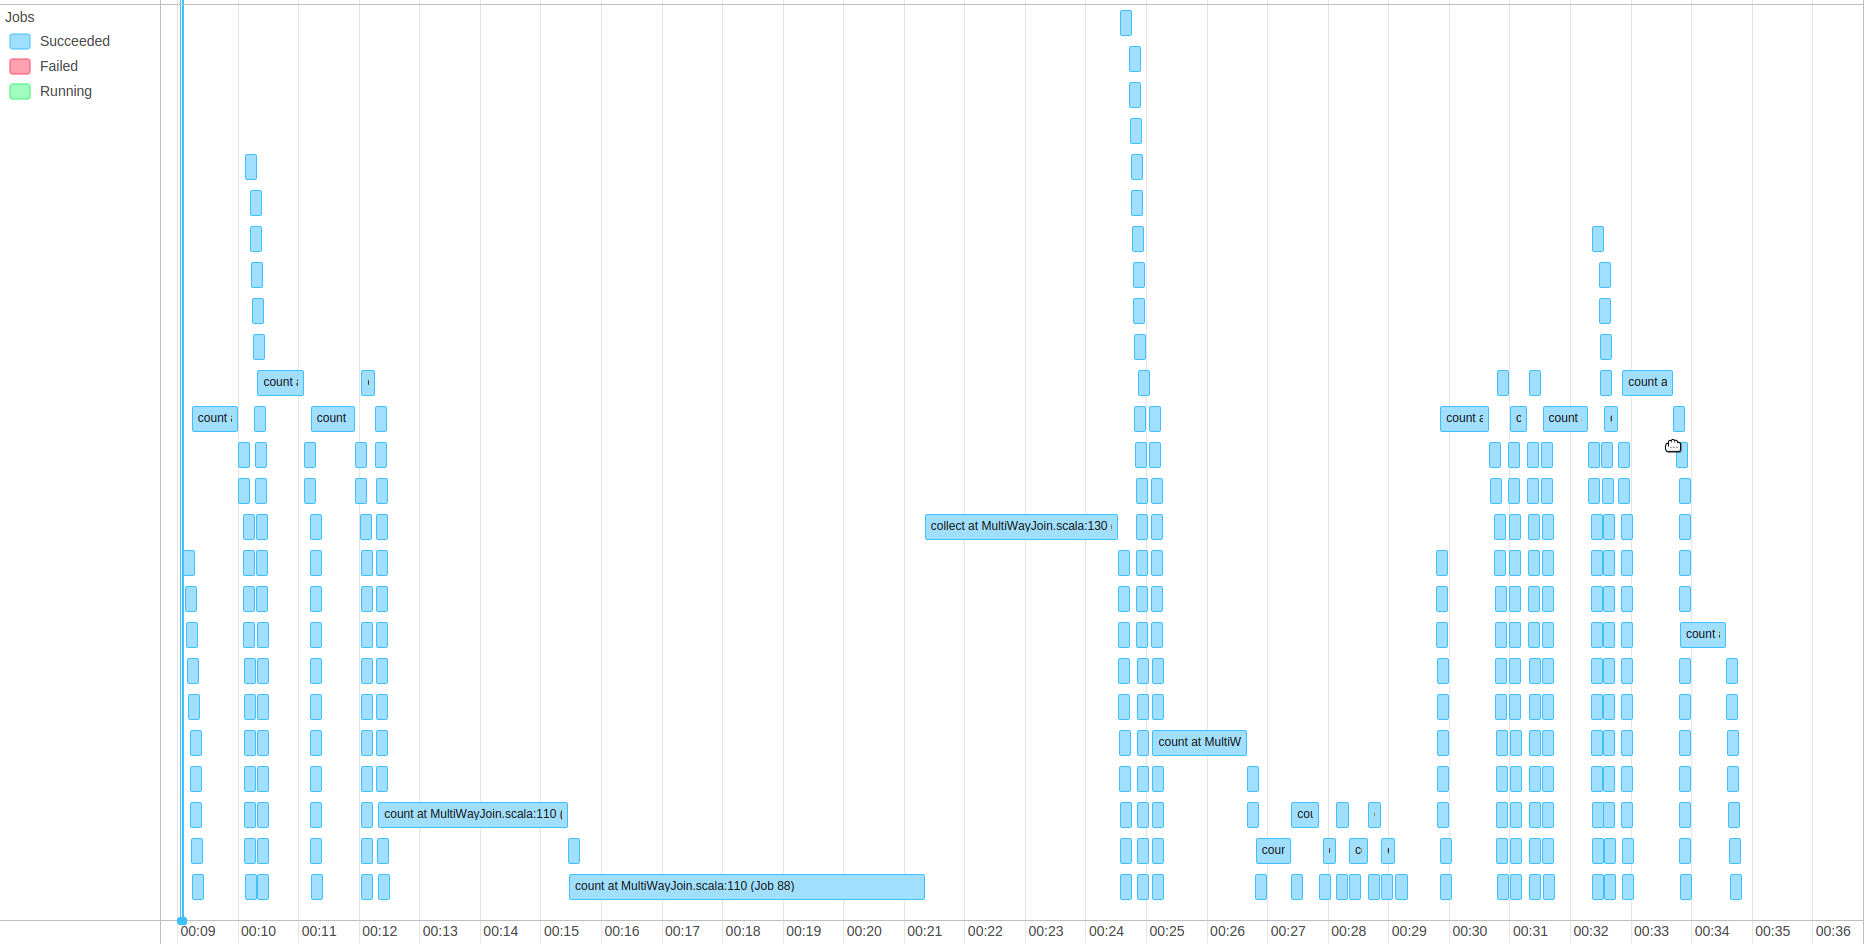
\includegraphics[width=0.8\textwidth]{img/alibaba-multi-jobs}
\end{figure}
\begin{figure}[h!]
  \caption{Job Flow of Modified Dan Suciu's Algorithm}
  \label{fig:alibaba-dan-jobs}
  \centering
    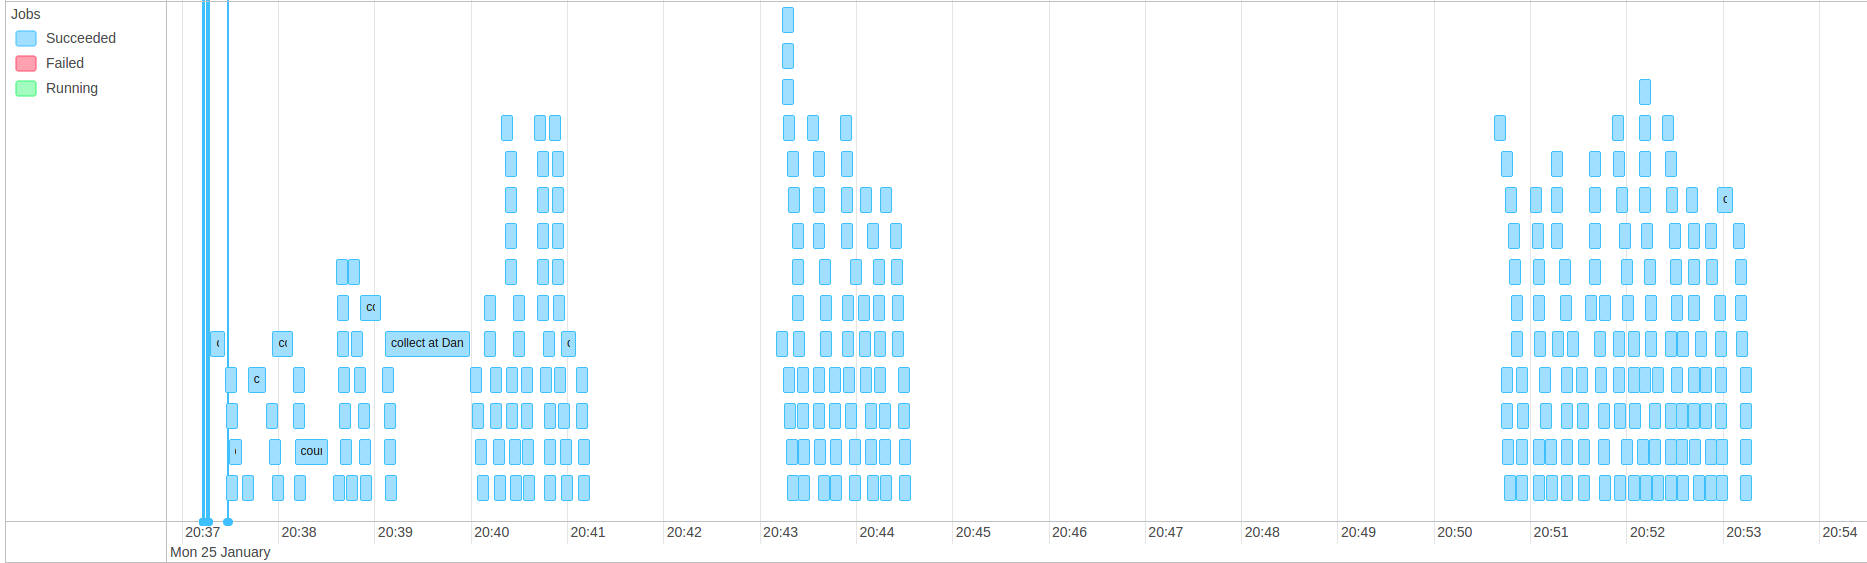
\includegraphics[width=0.8\textwidth]{img/alibaba-dan-jobs}
\end{figure}
\subsubsection{Cascaded 2-way Join}
By comparing those three charts, it can be found that there's no obvious bottleneck in the cascaded two-way join, which proves it to be the most scalable solution under Spark Context. The jobs taking more time are the `count' jobs in process graph \ref{fig:two-way-join-spark}. As Spark is of the lazy-evaluation model, it cannot be concluded that it's the `count'  task that taking so much time. By looking deeper into tasks of the `count' job in figure \ref{fig:alibaba-two-tasks}, it turns out that the full shuffle phases such as `subtract' and `distinct' costs the most time in `count' job. 
\subsubsection{Multi-way Join}
With respect to the Multi-way Join, we can see more obvious bottlenecks of `count' and `collect' jobs. During those jobs, edges distributed to different processors are merged in each task, which could result in huge blocking times as discussed in the previous section.
\begin{figure}[h!]
  \caption{Tasks of Count Job}
  \label{fig:alibaba-two-tasks}
  \centering
    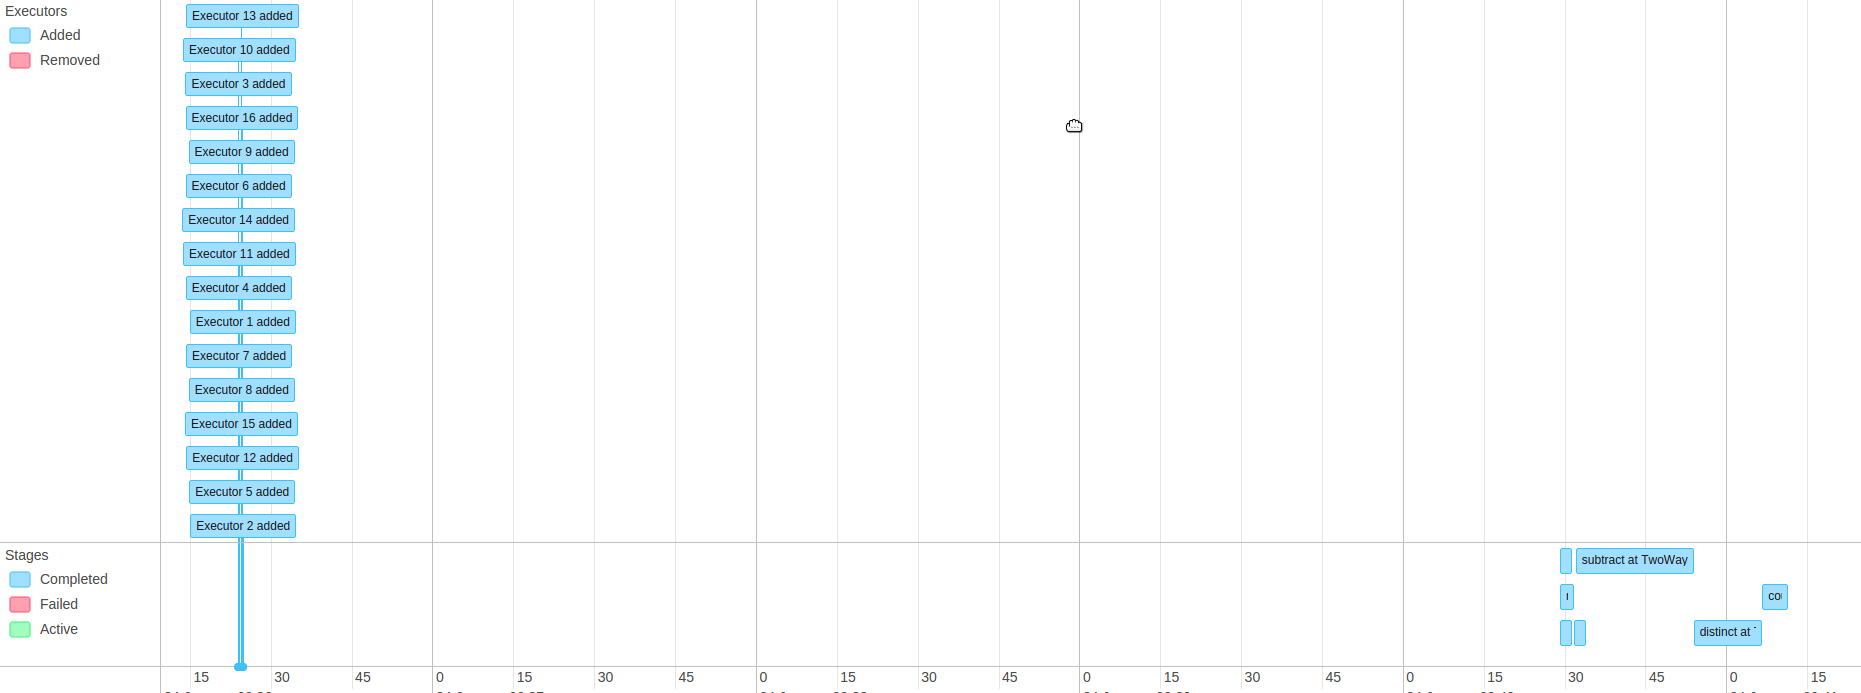
\includegraphics[width=1.0\textwidth]{img/alibaba-two-tasks}
\end{figure}
\subsubsection{Dan Suciu's Algorithm}
The blank parts in the chart of Dan Suciu's algorithm represent the time spent on the driver side. It takes more than half of the total time. On the executors' side, every second there are an almost same number of jobs running at the same time, which indicates the high parallelism. So in the next chapter, we will discuss the optimization of Dan Suciu's algorithm by reducing the size of global accessible graph (GAG) collected to the driver, thus reducing the computation time on the driver side.
\section{Data Shuffle Size}
The relation between the number of executors and shuffle size is included in diagram \ref{fig:two-way-join-shuffle}. As shuffle write size equals the sum of local shuffle read and remote shuffle read, we only show shuffle read data exchanged in it.  When we increase the number of workers, the remote read becomes larger. Finally, in the case of 64 workers, most of the shuffle read happens remotely, which is natural since with more workers added, less data will be local, and the probability of data exchange increases consequently.
\begin{figure}[h!]
  \caption{Shuffle Size of Two-Way Join}
  \label{fig:two-way-join-shuffle}
  \centering
    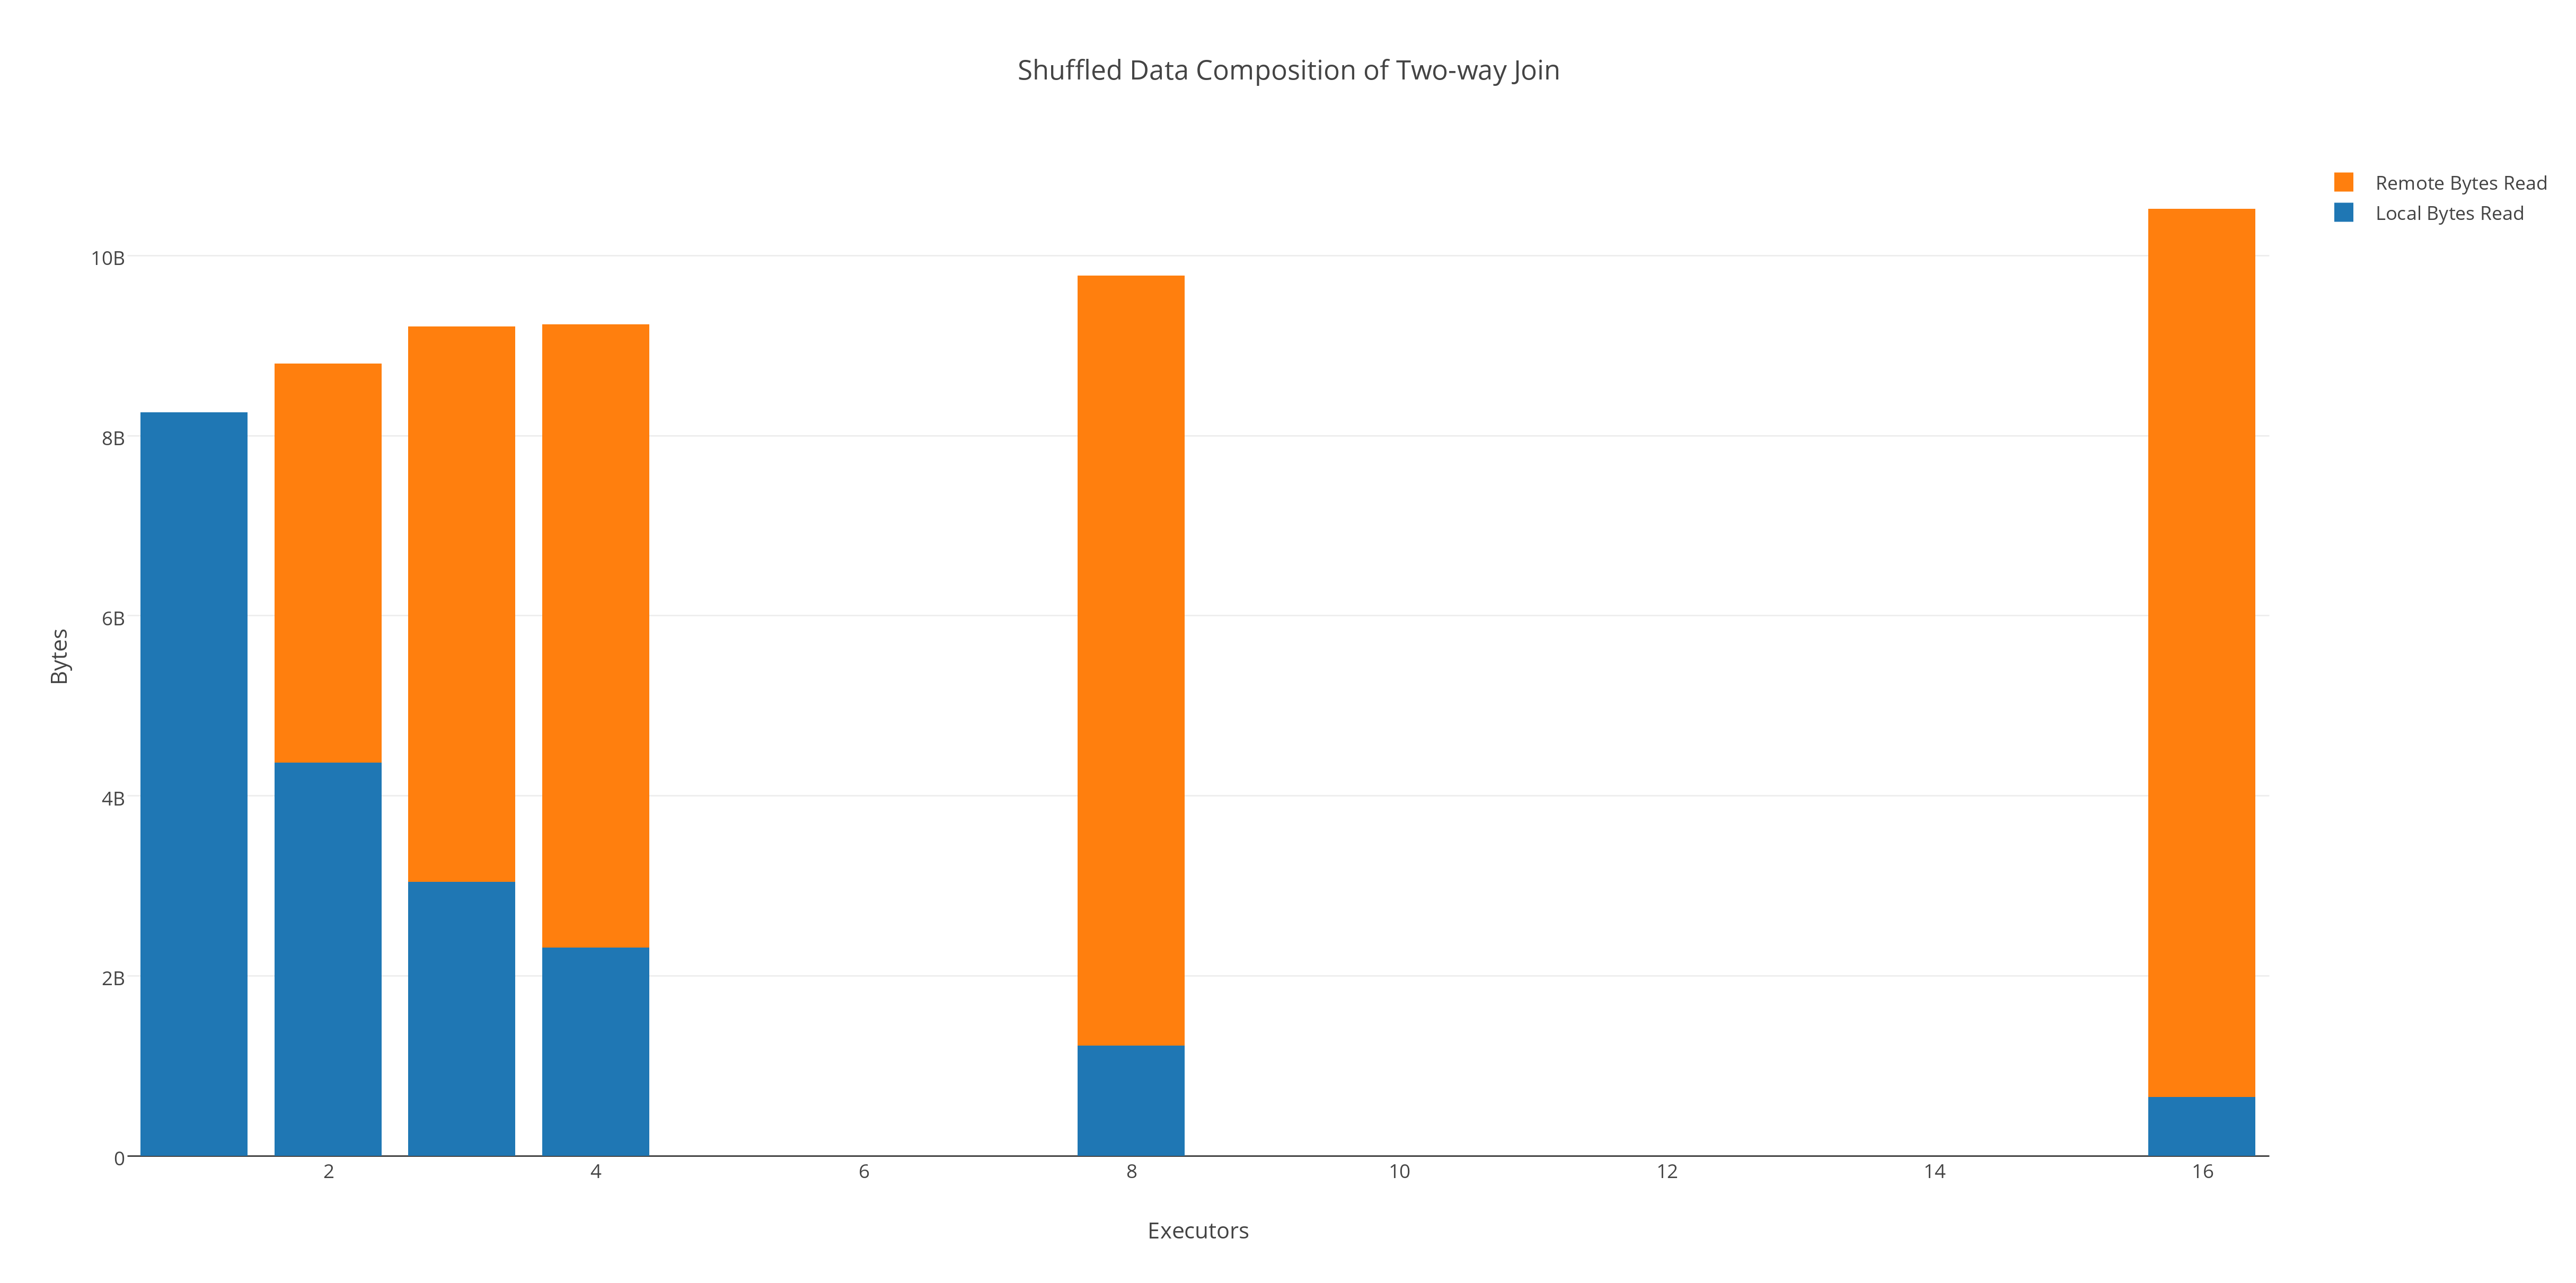
\includegraphics[width=1.0\textwidth]{img/Two-Way-Join-Shuffle-Data}
\end{figure}
\begin{table}[]
\centering
\caption{Shuffle Data Size of 3 Algorithms}
\label{Alibaba-Shuffle-Size}
\begin{tabular}{l|ll|ll|ll|}
   & \multicolumn{2}{c|}{2-way} & \multicolumn{2}{c|}{Multi-way} & \multicolumn{2}{c|}{Dan Scuciu} \\ \cline{2-7} 
   & Local         & Remote        & Local      & Remote      & Local          & Remote         \\ \hline
4  & 1.412 GB        & 5.534 GB        & 2.348 GB      & 7.502 GB        & 87,000 KB               & 252103 KB               \\
8  & 0.916 GB          & 6.182 GB         & 1.360 GB     & 9.273 GB        & 56,842 KB              & 374,842 KB              \\
16 & 0.424 GB          & 7.025 GB         & 0.623 GB       & 10.209 GB       & 37,341 KB              & 578,899 KB              \\
32 & 0.239 GB          & 7.903 GB         & 0.562 GB       & 10.767 GB       & 31,435 KB              & 955,104 KB             
\end{tabular}
\end{table}
\\Figure \ref{Alibaba-Shuffle-Size} compares the total data shuffled size for different algorithms. Comparing to other two algorithms, the shuffle size of Dan Suciu's algorithm can almost be ignored. Although multi-way join only shuffles once and process the local reduce task then, it still shuffles more bytes than cascaded two-way join.
\\However, if we look into more details in shuffle size of all tasks, the following findings can explain why multi-way join didn't improve the shuffle size:
\begin{enumerate}
    \item In the top 10 tasks of Cascaded 2-way Join that shuffle write most bytes, the executors only shuffle 700MB at most and those of the other tasks are around 300MBs. All of them are full shuffle tasks like `subtract' or `distinct'.
    \item With regards to the top 10 tasks of Multi-way Join that shuffle write most bytes, one of them shuffles 4GB , which is almost half of the whole shuffle write volume. And this task is `subtract' task, which is only triggered when dealing with queries with recurrence. This means the Multi-way Join shuffles much more than cascaded 2-way in the extreme case. Besides, all tasks that shuffle more than 100MB are relevant to the `subtract' or `distinct' operation when there is recurrence in the query.
    \item None of those tasks which dispatches states to Reduce tasks costs more than 100MB.
\end{enumerate}
The phenomenon is irrelevant to the number of workers as those bottleneck tasks are all full shuffle phases, which transmit the almost same amount of data despite the number of executors.
% \section{Memory Usage}
% As a trade-off, the multi-way join uses less memory as it doesn't need to cache intermediate results between iterations like cascaded two-way join. The peak memory usage of the two algorithms can be found in table \ref{peak-memory}
% \begin{table}[h!]
% \centering
% \caption{Peak Memory Usage of 2-way and Multi-way Join}
% \label{peak-memory}
% \begin{tabular}{lll}
% executors & cascaded two-way join & multi-way join \\
% 4         & 10.6 GB               & 6.8 GB         \\
% 8         & 19.9GB                & 7.5 GB         \\
% 16        & 27.5GB                & 8.2 GB         \\
% 32        & 32.2GB                & 8.7GB         
% \end{tabular}
% \end{table}

\section{Summary}
In this chapter, we run the Cascaded 2-way Join, Multi-way Join and modified Dan Suciu's algorithm against the Alibaba Benchmark and seek for some interesting findings. The measurements are conducted for metrics including running time, time stack and shuffle size. The following is the summary of observations:
\begin{enumerate}
    \item Cascaded 2-way Join is the most scalable solution of the three algorithms as the tasks are evenly distributed, and executors are blocked for the least time.
    \item Multi-way Join reduces shuffled size for simple queries. However, the shuffle size grows super fast when it deals with a query that contains recurrence.
    \item Dan Suciu's Algorithm seldom conducts shuffle, and it's limited by driver computation.
\end{enumerate}